
% \item \emph{ACC}: com um conjunto de quatro distâncias $D = {1, 3, 5, 7}$ e a distância tabuleiro de xadrez $D_8(p,q) = Max(|x-s|, |y-t|)$ entre os pixeis $p(x,y)$ e $q(s,t)$;
% \item \emph{BIC}: com uma vizinhança de quatro pixels;
% \item \emph{CCV}: adotando um valor de $\mathit{threshold} = 25$ para a classificação dos pixels entre coerentes e incoerentes;
% \item \emph{Haralick-6}: o pixel vizinho para o qual computar a matriz de correlação foi definido como sendo o pixel à direita.

%%%%%%%%%%%%%%%%%%%%%%%%%%%%%%%%%%%%%%%%%%%%%%%%%%%%%%%%%%%%%%%%%%%%%%%%%%%%%%%%
\section{Considerações Iniciais}

Os resultados encontrados ao rebalancear classes a partir da geração de imagens artificiais são apresentados neste capítulo. Para cada experimento realizado, são descritos: o protocolo utilizado (i.e. base de imagens e os métodos de conversão para escala de cinza e extração de características), os resultados encontrados e a discussão da relevância de tais resultados.

Foram realizados diversos experimentos direcionados a explorar o rebalanceamento com métodos de processamento, para melhorar a acurácia da classificação de bases de imagens. Como entrada são utilizadas imagens provenientes de diversas coleções disponíveis na literatura. Como resultado, são calculadas medidas estatísticas da classificação dessas bases de imagens após o rebalanceamento destas. Tal processamento é realizado antes da extração de características, e portanto no campo visual. Espera-se que os resultados encontrados proporcionem melhoras na etapa subsequente de classificação.

\meutodo{Nesse capítulo, falta ainda discutir melhor os resultados.}

%%%%%%%%%%%%%%%%%%%%%%%%%%%%%%%%%%%%%%%%%%%%%%%%%%%%%%%%%%%%%%%%%%%%%%%%%%%%%%%%

\section{Experimentos}

Essa seção descreve os resultados encontrados ao rebalancear as classes de imagens aplicando os processamentos -- descritos no Capítulo \ref{cap:metodo} -- nas imagens originais. As imagens geradas são então utilizadas como treinamento da classe minoritária. A Figura \ref{fig:fluxo} destaca o fluxo de operações realizadas para a análise do impacto da geração de imagens no rebalanceamento de classes. O mesmo protocolo de conversão para escala de cinza, extração de características e classificação foi seguido para três sub-experimentos: base desbalanceada; base rebalanceada com interpolação dos vetores de características (método SMOTE); e base rebalanceada com a geração artificial de imagens. Alguns experimentos foram realizados com bases de imagens originalmente balanceadas. Para tais casos, foi necessário desbalancear a base para testar o rebalanceamento.

\begin{figure}[!htbp]
\centering
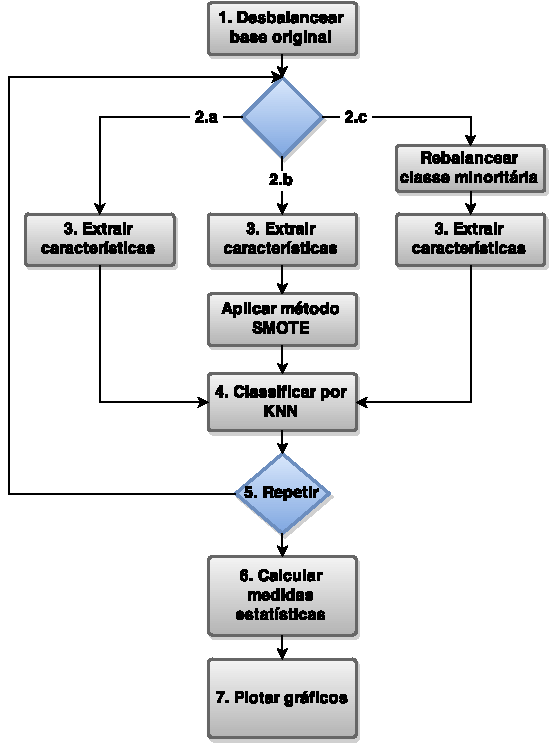
\includegraphics[scale=1.1]{\detokenize{figuras/flow_main.pdf}}
\caption[Fluxo de operações para obtenção dos resultados do rebalanceamento de classes]{Fluxo de operações para obtenção dos resultados do rebalanceamento de classes. \textit{Fonte:~Elaborado pela autora.}}
\label{fig:fluxo}
\end{figure}

Procurando estabilidade dos resultados obtidos com a geração das imagens artificiais, foi identificada a necessidade de controlar a remoção de imagens da base no momento da criação da base desbalanceada. Assim, os resultados foram obtidos a partir de uma forma de validação \textit{K-fold} com o objetivo de prover mais robustez ao sistema. A Figura \ref{fig:folds} ilustra como tal validação é realizada, utilizando como exemplo uma base com duas classes de imagens. Primeiramente as imagens são separadas de forma aleatória em $k = 5$ \textit{folds} em cada classe. Em seguida, as duas classes compõem 40 configurações, consistindo em todas as possibilidades de: um fold para teste e os outros como treino para a classe que permanecerá balanceada; e um de teste e apenas um de treino para a classe que os métodos de processamento irão rebalancear. Tal validação é repetida para todas as classes, ou seja, cada classe tem a possibilidade de ser a minoritária. Se originalmente a base é naturalmente desbalanceada, um \textit{fold} é utilizado para teste e os demais como treino para todas as classes.

\begin{figure}[!htbp]
\centering
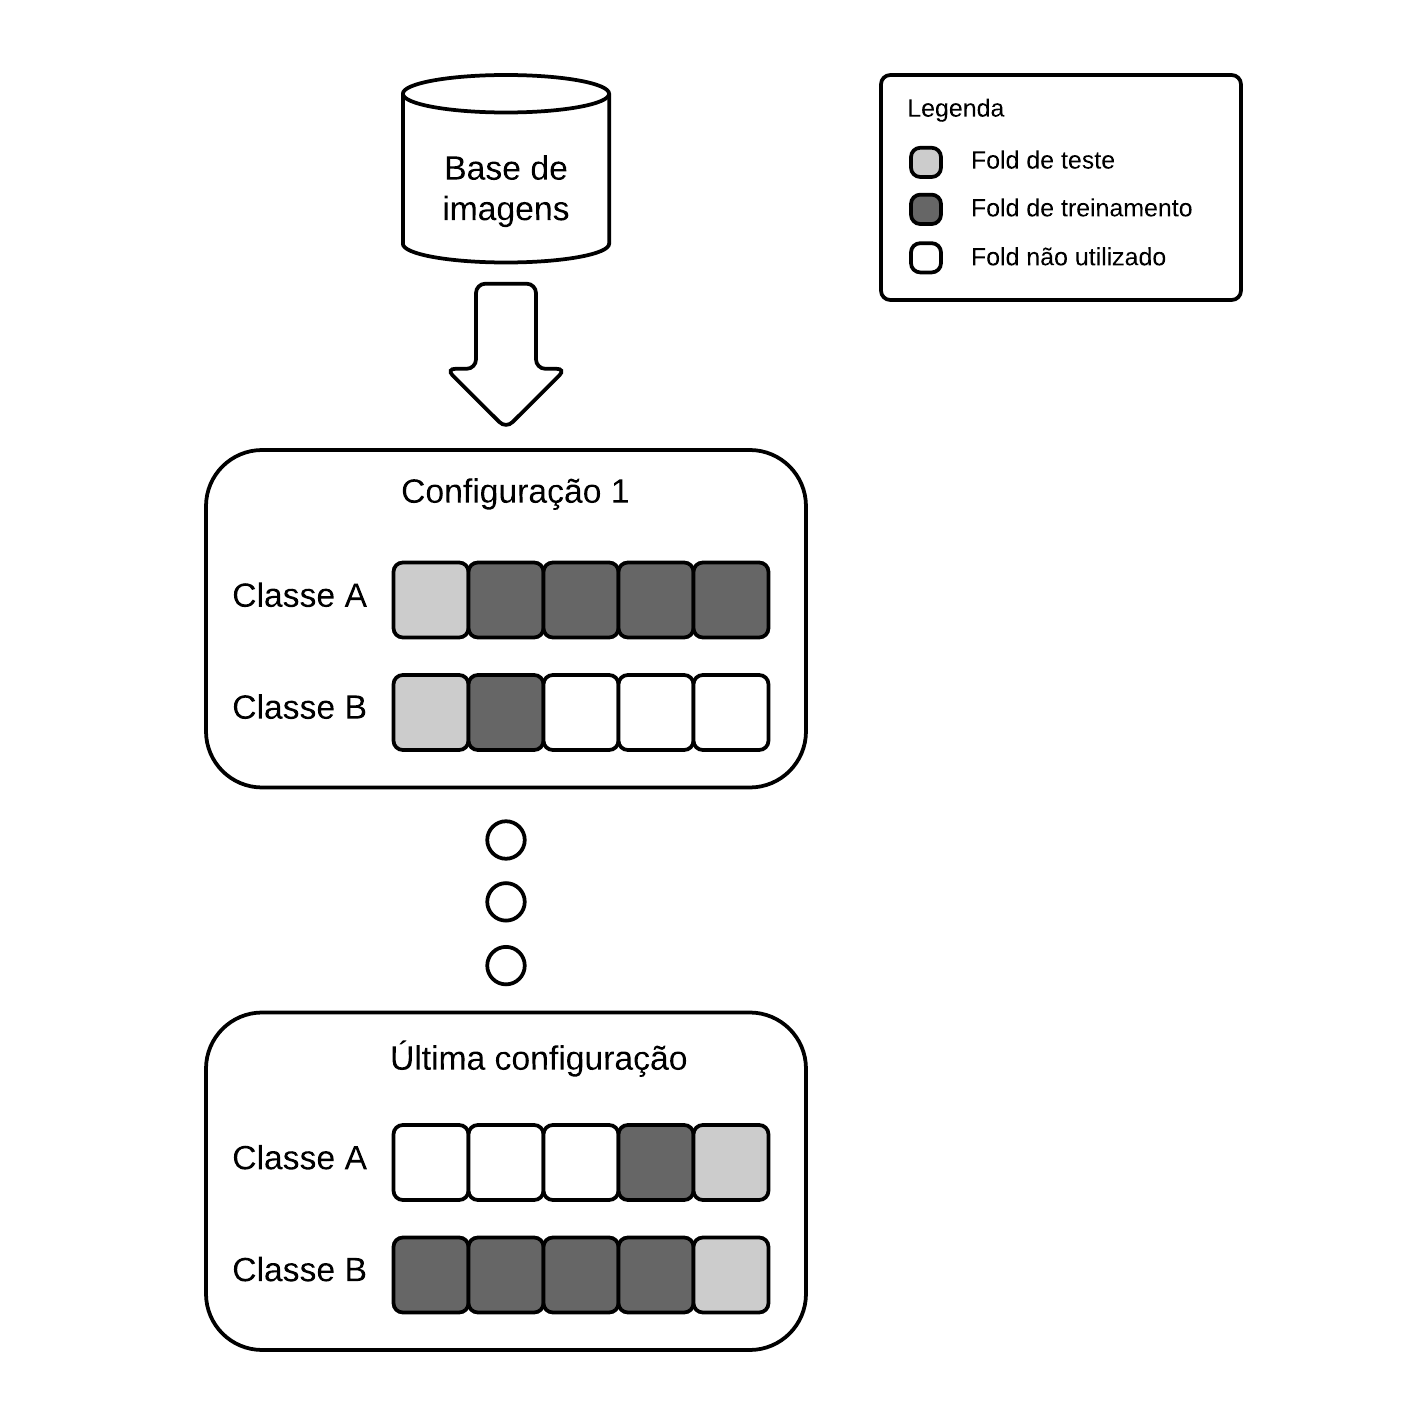
\includegraphics[scale=0.3]{\detokenize{figuras/folds_chart.png}}
\caption[]{\textit{Fonte:~Elaborado pela autora.}}
\label{fig:folds}
\end{figure}

\meutodo{Tenho que escrever o caption}

A medida estatística mais comum para avaliação é a razão do número de acertos pela quantidade de imagens testadas. Essa medida, conhecida por \underline{acurácia}, pode não refletir propriamente os resultados em um cenário de bases desbalanceadas. Isso se deve ao fato de que se a classe minoritária não obtiver nenhum resultado correto e a classe majoritária tiver 100\% de acertos, tal acurária poderá ser muito alta, mesmo considerando que nenhuma imagem da classe minoritária foi corretamente classificada. Dessa forma, considera que os erros são igualmente importantes. Mas em se tratando de bases desbalanceadas, deve-se diferenciar o erro em, por exemplo, diagnosticar um paciente doente -- classe minoritária -- como sendo saudável e um paciente saudável -- classe majoritária -- como estando doente \cite{Batista2004}. No primeiro caso, o paciente corre risco de diagnóstico tardil, enquanto o paciente saudável realiza outros testes para refutação.

Pode-se estender essa medida obtendo-se a \underline{acurácia $k$-fold}: medida de acerto baseada na divisão do conjunto de objetos em teste e treinamento, realizando a repetição dos experimentos $n$ vezes e obtendo a média e o desvio padrão. A acurácia de cada experimento é obtida por

    \begin{equation*}
      Acc = 1 - \frac{\sum_{i=1}^{c} E(i)}{2c},
    \label{eq:Accuracy}
    \end{equation*}

    \noindent  que considera problemas de desbalanceamento de classes, onde $c$ é o número de classes e $E(i) = e_{i,1} + e_{i,2}$ é o erro relativo a $c$, calculado por

    \begin{equation*}
      e_{i,1} = \frac{FP(i)}{N-N(i)} \,\,\,\,\, \text{ e } \,\,\,\,\, e_{i,2} = \frac{FN(i)}{N(i)}, i=1,...,c,
    \label{eq:Errors}
    \end{equation*}
   \noindent onde $FN(i)$ são os exemplos pertencentes a $i$ e incorretamente classificados (falsos negativos), e $FP(i)$ são os exemplos erroneamente rotulados como~$i$ (falsos positivos).

% consideramos positivos a minoritaria

Uma outra medida, que pode efetivamente avaliar a performance de classificação em cenários desbalanceados, é a \underline{medida-F1} (conhecida como \textit{F1-Measure} ou \textit{F1-Score}):

\begin{equation*}
  F1 = 2 \frac{PR}{P+R}.
\end{equation*}

Essa medida combina precisão e revocação como medida de efetividade da classificação \cite{Garcia2009}. A precisão é a medida da exatidão:

\begin{equation*}
  P = \frac{VP}{VP + FP},
\end{equation*}

\noindent onde $VP$ são os exemplos positivos corretamente classificados. Dos exemplos classificados como positivos, essa medida indica quantos realmente são. Ao mesmo tempo, a revocação é a medida de completude. Essa métrica indica quantos exemplos positivos foram corretamente classificados. Pode ser determinada por:

\begin{equation*}
  R = \frac{VP}{VP + FN}.
\end{equation*}

A partir dessas medidas estatísticas, o teste HSD de Tukey pode ser utilizado para determinar se há diferença significativa em uma amostra de resultados gerados.

\meutodo{Explicar melhor? aonde colocar p-value < 0,05 e a hipótese nula?}

% A partir dessas medidas, o \underline{teste estatístico de Friedman} pode ser usado para determinar se há diferença significante em uma amostra de resultados gerados \cite{friedman2010}. As performances dos algoritmos são analisados e um \textit{rank} é atribuído para cada conjunto de dados. Ele considera que a hipótese nula a ser testada é que não há diferença estatística relevante entre as observações. Para analisar se o teste da hipótese é significativo, pode ser utilizado o \underline{p-valor}, que indica o quão estatisticamente significante o resultado é: quanto menor o seu valor, maior a evidência contra a hipótese nula (geralmente o limiar utilizado é de 0,05).

A seguir, para cada experimento realizado são descritos: a base de imagens utilizada; o protocolo e parâmetros adotados; e por fim os resultados obtidos a partir de seu uso são mostrados e discutidos.

%%%%%%%%%%%%%%%%%%%%%%%%%%%%%%%%%%%%%%%%%%%%%%%%%%%%%%%%%%%%%%%%%%%%%%%%%%%%%%%%
\FloatBarrier
\subsection{Experimento 1: duas classes bem discriminadas}

Neste experimento foram utilizadas duas classes com cores bem distintas entre elas, ou seja, de fácil diferenciação. Por tal razão, um sub-experimento de visualização foi realizado para análise do espaço de características. Como o foco é na visualização de tal espaço, é relevante ter o modelo do espaço ideal das classes balanceadas. Por conta disso, esse experimento em específico não trata de uma base naturalmente desbalanceada.

%-------------------------------------------------------------------------------
\subsubsection{Protocolo}
\begin{enumerate}
\item \textbf{Imagens originais}: classes \emph{Cavalo} e \emph{Elefante} da base de imagens Corel, exemplificadas na Figura \ref{fig:resultados:1:base} \cite{Wang2001}. A principal característica dessas imagens é a diferença de cores. Apesar de haverem casos de confusão, são classes que podem ser consideradas bem discriminadas.

\begin{minipage}{\linewidth}
\begin{figure}[H]
  \begin{center}
    \subfloat{
      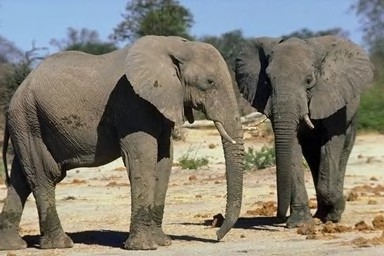
\includegraphics[width=0.45\linewidth]{\detokenize{figuras/corel_original4.jpg}}
    }
    \subfloat{
      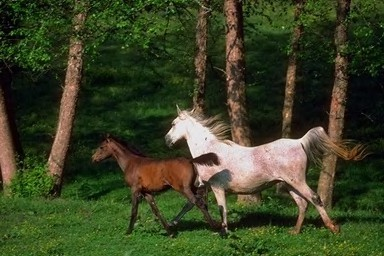
\includegraphics[width=0.45\linewidth]{\detokenize{figuras/cavalo-original2.png}}
    }

    \caption[Classes \emph{Cavalo} e \emph{Elefante} utilizadas neste experimento. São duas classes bem discriminadas com 100 imagens cada, originalmente da base de imagens Corel.]{Classes \emph{Cavalo} e \emph{Elefante} utilizadas neste experimento. São duas classes bem discriminadas com 100 imagens cada, originalmente da base de imagens Corel. \textit{Fonte:~\cite{Hu2013}.}}
    \label{fig:resultados:1:base}
\end{center}
\end{figure}
\end{minipage}

\item \textbf{Desbalanceamento}: para o sub-experimento de visualização, cada classe foi dividida em 50\% para treino e 50\% para teste, de maneira aleatória. Após, a classe \emph{Cavalo} sofreu remoção de 50\% do seu conjunto de treino, tornando-a desbalanceada. Já para a análise estatística do experimento, todas as 40 configurações de folds com $k=5$ foram realizadas (padronização anteriormente descrita na Figura~\ref{fig:folds}).

\item \textbf{Método para geração artificial}: para a visualização do espaço de características foi utilizado o método de mistura de duas imagens originais, exemplificado na Figura~\ref{fig:mistura}. Para a análise do boxplot de \textit{f1-scores}, todas as gerações foram testadas e os resultados são reportados a seguir.

\begin{minipage}{\linewidth}
\begin{figure}[H]
  \begin{center}
    \subfloat[Original]{
      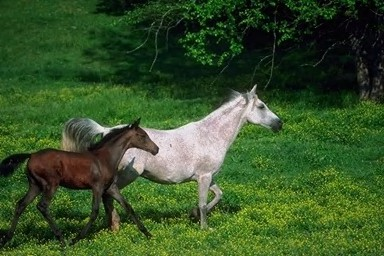
\includegraphics[width=.33\linewidth]{\detokenize{figuras/cavalo-original.png}}
    }
    \subfloat[Original]{
      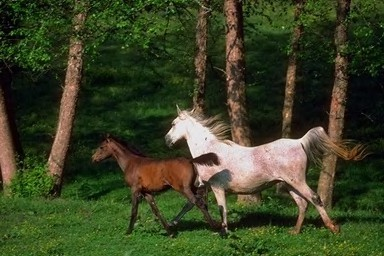
\includegraphics[width=.33\linewidth]{\detokenize{figuras/cavalo-original2.png}}
    }
    \subfloat[Mistura]{
      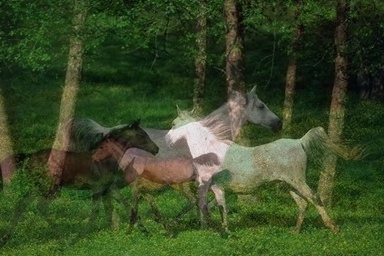
\includegraphics[width=.33\linewidth]{\detokenize{figuras/cavalo-blend.png}}
    }
    \caption[Exemplo da geração artificial de imagens com o método de mistura para as classes \emph{Elefante} e \emph{Cavalo} da Corel-1000.]{Exemplo da geração artificial de imagens com o método de mistura para as classes \emph{Elefante} e \emph{Cavalo} da Corel-1000. \textit{Fonte:~Elaborado pela autora.}}
    \label{fig:mistura}
\end{center}
\end{figure}
\end{minipage}

\item \textbf{Conversão em escala de cinza}: método \emph{Intensidade'} para a visualização. Todas as combinações de extração e conversão em escala de cinza foram testadas, portanto todos os métodos de conversão foram utilizados.

\item \textbf{Extração de características}: classificação de pixels de borda e interior (BIC) para a visualização. Todos os métodos de extração foram testados para a análise estatística.

\item \textbf{Classificação}: Inicialmente o classificador \textit{Naive Bayes} foi explorado, apresentando melhora na acurácia ao apenas replicar as imagens. Esse comportamento não é desejado em um classificador para a avaliação de rebalanceamento de classes. Por essa razão e por permitir uma análise da melhora no comportamento da classificação, o classificador supervisionado KNN com $K=1$ (para mais detalhes ver Seção~\ref{sec:knn}) foi utilizado.

\item \textbf{Projeção multidimensional}: dois componentes principais encontrados ao aplicar PCA (Seção~\ref{sec:pca}) nos vetores de características para redução de dimensionalidade foram projetados.
\end{enumerate}

%-------------------------------------------------------------------------------
\FloatBarrier
\subsubsection{Visualização}

As classes \emph{Elefante} e \emph{Cavalo} possuem 100 imagens cada. O primeiro passo foi remover imagens de uma das classes, tornando a base desbalanceada. Na Figura~\ref{fig:desbalanceado} está ilustrada a remoção de 50\% das imagens de treino da classe \emph{Cavalo}, originalmente balanceada. Essa e as próximas projeções desta seção foram obtidas com a técnica para redução de dimensionalidade PCA, descrita na Seção~\ref{sec:pca}, e são referentes aos dois componentes principais com maiores autovalores.

\begin{figure}[!htbp]
  \begin{center}
    \subfloat[Original]{
      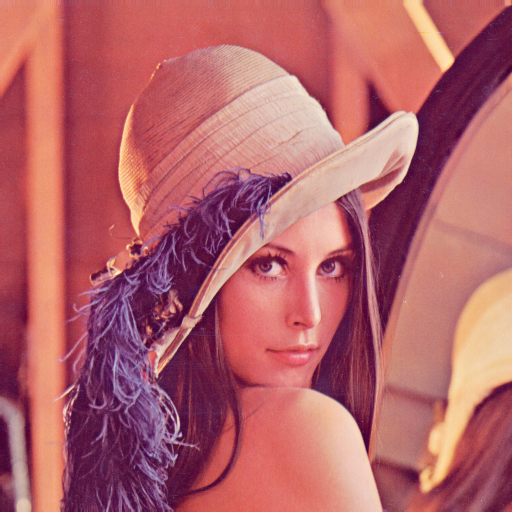
\includegraphics[width=.5\linewidth]{\detokenize{figuras/visualizacao/original.png}}
    }
    \subfloat[Desbalanceado]{
      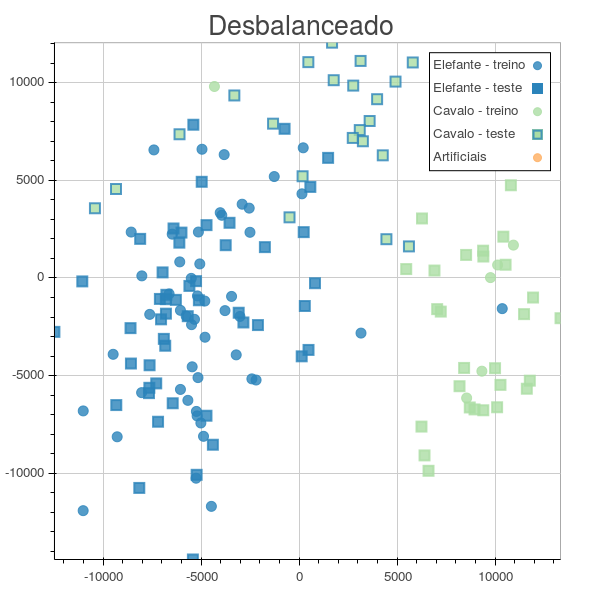
\includegraphics[width=.5\linewidth]{\detokenize{figuras/visualizacao/desbalanceado-fixed.png}}
    }
    \caption[À esquerda a projeção dos dois componentes principais obtidos com a aplicação de PCA nas classes \emph{Elefante} -- em azul -- e \emph{Cavalo} -- em verde. À direita, as mesmas classes após a remoção de 50\% das imagens de treino da classe \emph{Cavalo}. A diferença dos marcadores consiste na definição de imagens para treino e teste não existente nas classes originais.]{À esquerda a projeção dos dois componentes principais obtidos com a aplicação de PCA nas classes \emph{Elefante} -- em azul -- e \emph{Cavalo} -- em verde. À direita, as mesmas classes após a remoção de 50\% das imagens de treino da classe \emph{Cavalo}. A diferença dos marcadores consiste na definição de imagens para treino e teste não existente nas classes originais. \textit{Fonte:~Elaborado pela autora.}}
    \label{fig:desbalanceado}
\end{center}
\end{figure}

Os resultados da classificação dos três experimentos (desbalanceado, SMOTE e geração artificial) utilizando KNN com $K=1$ reportou que o \textit{f1-score} da geração de imagens utilizando o método de mistura teve um ganho satisfatório em relação ao rebalanceamento no espaço de características com o SMOTE (apresentado na Figura \ref{fig:resultados:1:vis}). Foi utilizado \emph{BIC} como método de extração de características e \emph{Intensidade'} como método de conversão em escala de cinza. Para essa combinação, a geração de imagens utilizando mistura se mostrou favorável e portanto a visualização do espaço de características apresenta esse método como geração.

\begin{figure}[!htbp]
  \begin{center}
      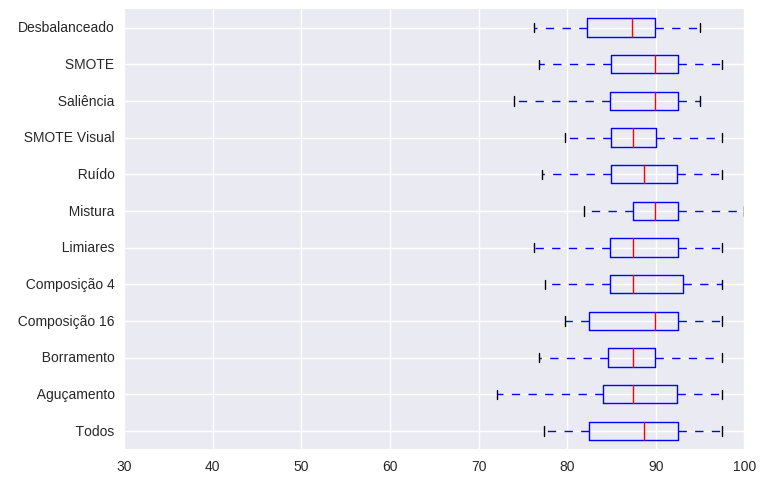
\includegraphics[width=\linewidth]{\detokenize{figuras/resultados/1/BIC_Intensity_elefante-cavalo.png}}
    \caption[Resultados de \textit{f1-score} para as classes \emph{Cavalo} e \emph{Elefante} da base Corel. Foi utilizado \emph{BIC} como método de extração de características e \emph{Intensidade'} como método de conversão em escala de cinza. Para essa combinação, a geração de imagens utilizando mistura se mostrou favorável.]{Resultados de \textit{f1-score} para as classes \emph{Cavalo} e \emph{Elefante} da base Corel. Foi utilizado \emph{BIC} como método de extração de características e \emph{Intensidade'} como método de conversão em escala de cinza. Para essa combinação, a geração de imagens utilizando \emph{mistura} se mostrou favorável. \textit{Fonte:~Elaborado pela autora.}}
    \label{fig:resultados:1:vis}
\end{center}
\end{figure}

% \meutodo{necessário a tabela reference aos F1-Scores da figura acima? está comentado}
% \begin{table}[!htbp]
% \centering
% \caption{Resultados de \textit{f1-score} para as classes \emph{Cavalo} e \emph{Elefante}, utilizando \emph{Intensidade'} como método para conversão em escala de cinza e \emph{BIC} para extração de características.}
% \label{fig:resultados:1:tabvis}
% \begin{tabular}{|l|c|c|}
% \hline
% \textbf{Intensidade' e BIC} & \textbf{Média} & \textbf{Desvio padrão} \\ \hline
% Todos                      & 88.07          & 5.30                   \\ \hline
% Aguçamento                 & 86.65          & 7.00                   \\ \hline
% Borramento                 & 87.17          & 5.10                   \\ \hline
% Composição 16              & 88.16          & 5.32                   \\ \hline
% Composição 4               & 88.12          & 5.45                   \\ \hline
% Limiares                   & 87.65          & 5.10                   \\ \hline
% Mistura                    & \textbf{88.84} & 5.03          \\ \hline
% Ruído                      & 87.95          & 5.75                   \\ \hline
% SMOTE Visual               & 87.69          & 5.28                   \\ \hline
% Saliência                  & 88.09          & 5.58                   \\ \hline
% SMOTE                      & 88.55          & 5.21                   \\ \hline
% Desbalanceado              & 85.82          & 5.69                   \\ \hline
% \end{tabular}
% \end{table}

Para verificar se a geração de imagens inseriu mais informação na classe minoritária do que apenas povoar os espaços entre os exemplos (i.e.\ SMOTE), a classe rebalanceada utilizando ambos métodos está demonstrada na Figura~\ref{fig:compara_vis_treino_fixed}. Em laranja estão representados os novos exemplos de treinamento, projetados no plano da base original balanceada.

\begin{figure}[!htbp]
  \begin{center}
    \subfloat[Smote]{      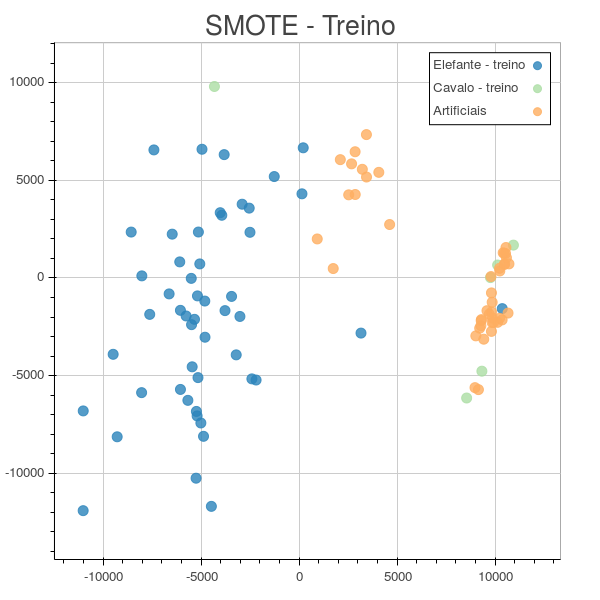
\includegraphics[width=.5\linewidth]{\detokenize{figuras/visualizacao/smote-treino-fixed.png}}
    }
    \subfloat[Geração artificial]{      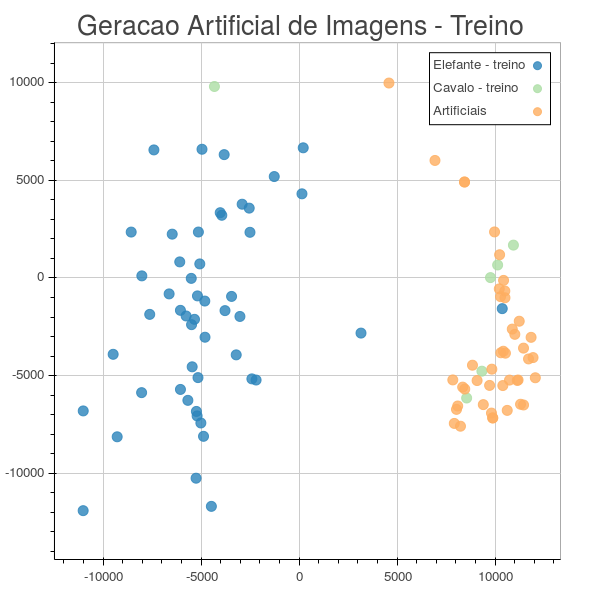
\includegraphics[width=.5\linewidth]{\detokenize{figuras/visualizacao/geracao-treino-fixed.png}}
    }
  \caption[Comparação dos exemplos de treinamento da geração com SMOTE e no campo visual. Em laranja estão representados os novos exemplos, projetados no plano da base original balanceada.]{Comparação dos exemplos de treinamento da geração com SMOTE e no campo visual. Em laranja estão representados os novos exemplos, projetados no plano da base original balanceada. \textit{Fonte:~Elaborado pela autora.}}
  \label{fig:compara_vis_treino_fixed}
  \end{center}
\end{figure}

Após o treinamento realizado com as novas imagens geradas e as originais, o conjunto de teste foi fornecido ao classificador 1-NN e o resultado das predições está ilustrado na Figura~\ref{fig:compara_vis_teste}. A cor no interior dos marcadores quadrados representa a classe real dos exemplos e a borda representa a classe predita pelo classificador. Nota-se que a melhoria na classificação com a geração de imagens fica visível e corresponde ao aumento do \textit{f1-score}.

\begin{figure}[!htbp]
  \begin{center}
    \subfloat[Smote]{
      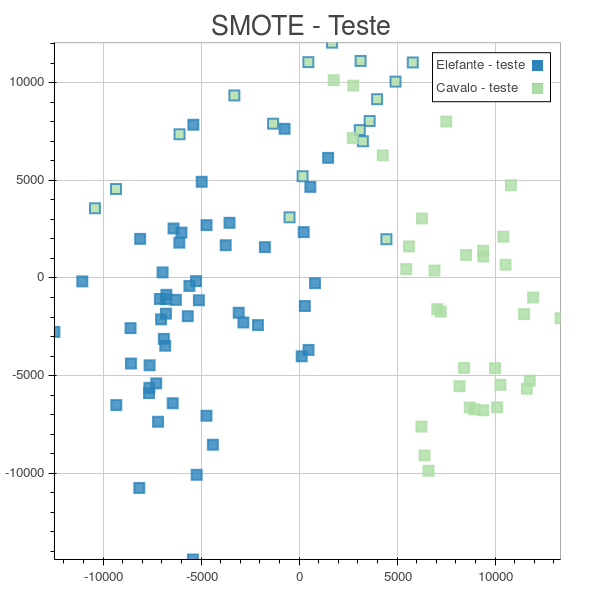
\includegraphics[width=.5\linewidth]{\detokenize{figuras/visualizacao/smote-teste-fixed.png}}
    }
    \subfloat[Geração artificial]{
      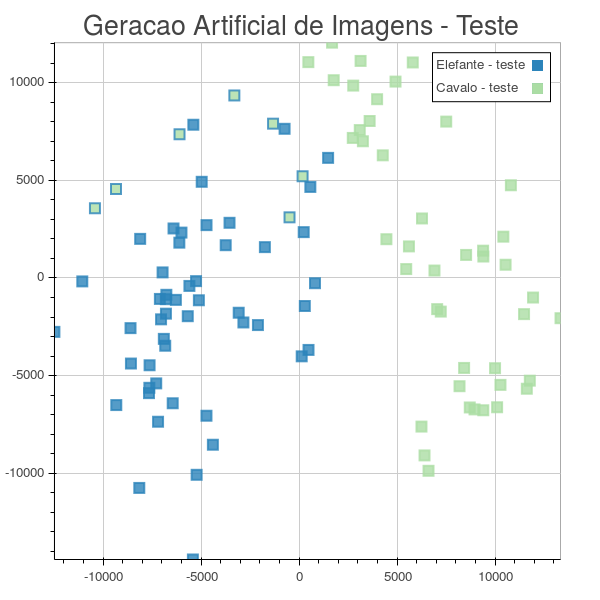
\includegraphics[width=.5\linewidth]{\detokenize{figuras/visualizacao/geracao-teste-fixed.png}}
    }
  \caption[Resultado do teste da classificação com 1-NN após o treinamento realizado com as bases rebalanceadas. A cor no interior dos marcadores quadrados representa a classe real dos exemplos e a borda representa a classe predita pelo classificador.]{Resultado do teste da classificação com 1-NN após o treinamento realizado com as bases rebalanceadas. A cor no interior dos marcadores quadrados representa a classe real dos exemplos e a borda representa a classe predita pelo classificador. \textit{Fonte:~Elaborado pela autora.}}
  \label{fig:compara_vis_teste}
\end{center}
\end{figure}

De uma forma geral, pode-se dizer que a geração de imagens melhorou a definição da classe minoritária e foi o método que mais se assemelhou à distribuição dos dados originais. Além disso, um dos problemas do SMOTE pode ser verificado nessas projeções: \textbf{ao realizar a interpolação dos vetores de características originais, exemplos podem ser criados em regiões do espaço que fazem parte da outra classe}. Ficou claro também que o método SMOTE não possui capacidade de extrapolar a sua região, como pode ser observado no grupo de exemplos gerados à direita do espaço de características. O SMOTE gerou novos elementos próximos a uma linha reta, enquanto a geração de imagens proporcionou uma abrangência maior em volta desse espaço, com maior dispersão.

Na Figura \ref{fig:region} é possível visualizar a região de decisão, observando suas modificações frente aos métodos. Pode ser observado que em ambas técnicas a região da classe minoritária apresenta-se melhor representada. Além disso, é possível verificar que o SMOTE ocasionou uma certa ``invasão'' do espaço de características da classe majoritária.

\begin{figure}[!htbp]
    \begin{center}
    \subfloat[Desbalanceado]{
      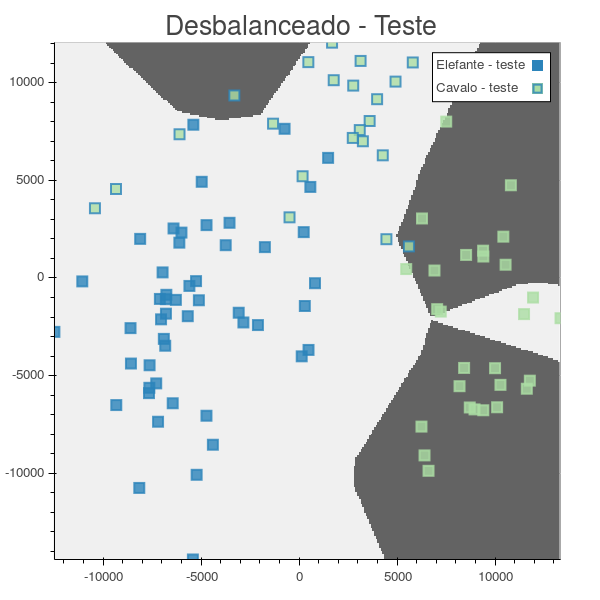
\includegraphics[width=.5\linewidth]{\detokenize{figuras/visualizacao/desbalanceado-teste-region.png}}
    }
    \end{center}
    \subfloat[Smote]{
      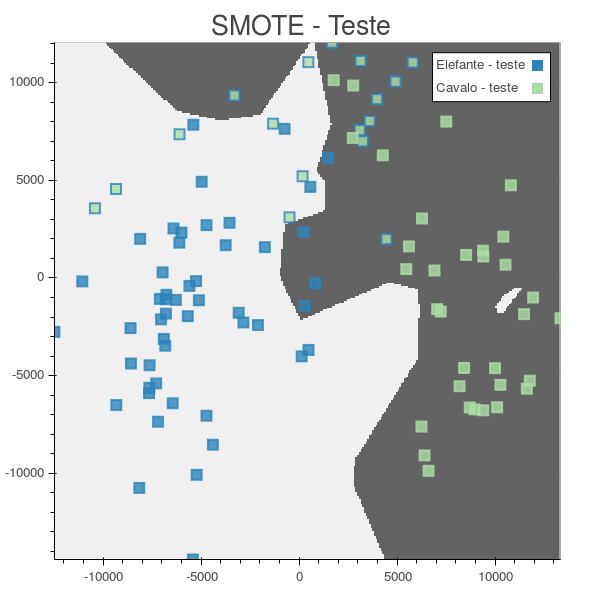
\includegraphics[width=.5\linewidth]{\detokenize{figuras/visualizacao/smote-teste-region.png}}
    }
    \subfloat[Geração artificial]{
      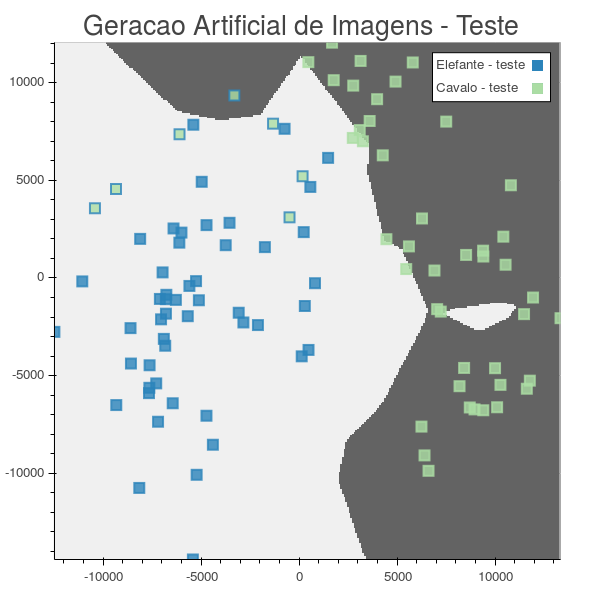
\includegraphics[width=.5\linewidth]{\detokenize{figuras/visualizacao/geracao-teste-region.png}}
    }
  \caption[Região de decisão com K-NN (K = 1). Pode ser observado que em ambas técnicas a região da classe minoritária apresenta-se melhor representada. Além disso, é possível verificar que o SMOTE ocasionou uma certa ``invasão'' do espaço de características da classe majoritária.]{Região de decisão com K-NN (K = 1). Pode ser observado que em ambas técnicas a região da classe minoritária apresenta-se melhor representada. Além disso, é possível verificar que o SMOTE ocasionou uma certa ``invasão'' do espaço de características da classe majoritária. \textit{Fonte:~Elaborado pela autora.}}
  \label{fig:region}
\end{figure}

Em todas as figuras anteriores relacionadas a essa visualização, os exemplos foram projetados no plano criado pelas suas componentes principais com maior autovalores da base original balanceada. Se após a geração de novos exemplos essas componentes forem recalculadas (Figura \ref{fig:compara_vis_treino}), pode-se notar que a geração de imagens artificiais proporciona a criação de um subespaço que melhor discretiza as classes, quando comparado com SMOTE ou com a base desbalanceada.

\begin{figure}[!htbp]
    \begin{center}
    \subfloat[Desbalanceado]{
      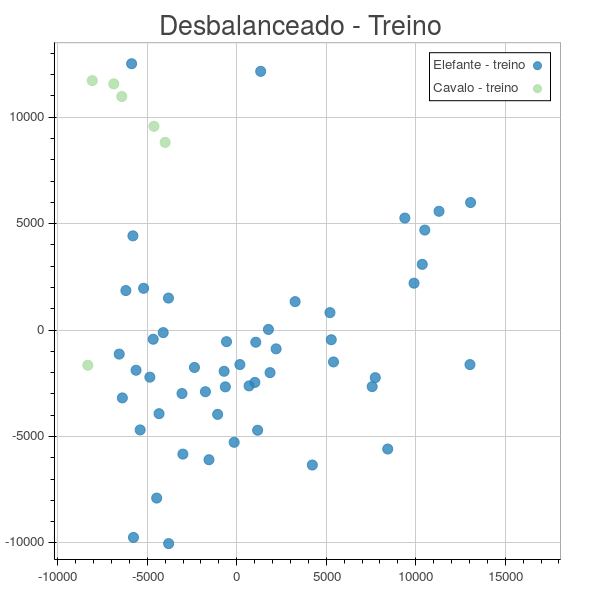
\includegraphics[width=.5\linewidth]{\detokenize{figuras/visualizacao/desbalanceado-treino.png}}
    }
    \end{center}
    \subfloat[Smote]{
      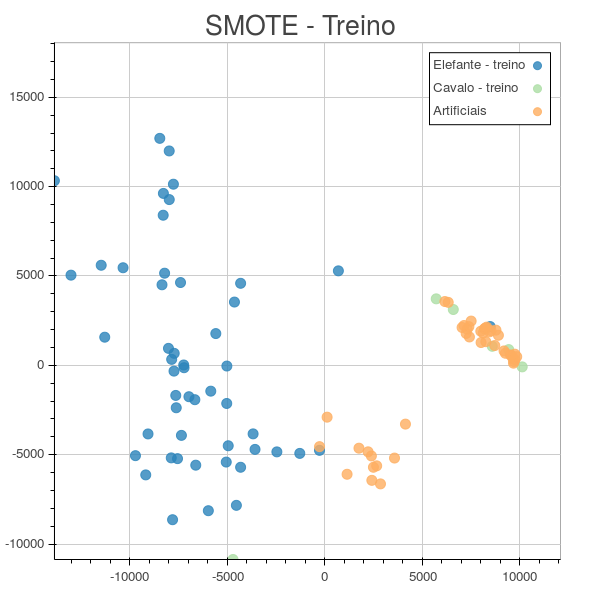
\includegraphics[width=.5\linewidth]{\detokenize{figuras/visualizacao/smote-treino.png}}
    }
    \subfloat[Geração artificial]{
      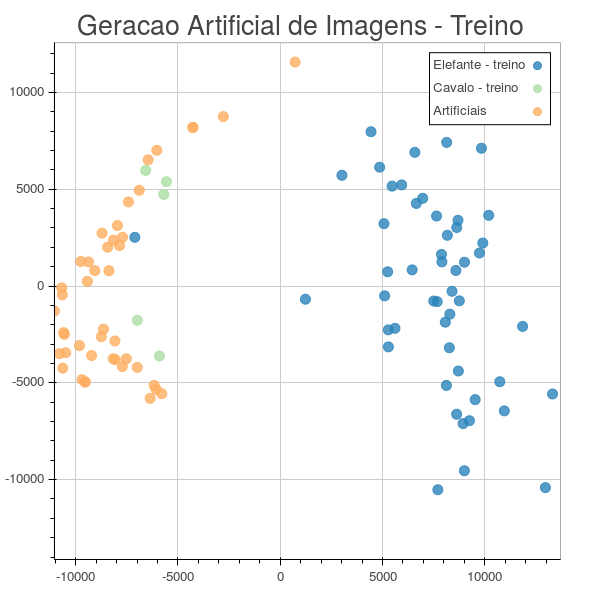
\includegraphics[width=.5\linewidth]{\detokenize{figuras/visualizacao/geracao-treino.png}}
    }
  \caption[Melhores subespaços encontrados após a geração de novos exemplos para o SMOTE e para a geração artificial de imagens, e após a remoção de imagens para a projeção dos dados desbalanceados. Pode-se notar que a geração de imagens artificiais proporciona a criação de um subespaço que melhor discretiza as classes, quando comparado com SMOTE ou com a base desbalanceada.]{Melhores subespaços encontrados após a geração de novos exemplos para o SMOTE e para a geração artificial de imagens, e após a remoção de imagens para a projeção dos dados desbalanceados. Pode-se notar que a geração de imagens artificiais proporciona a criação de um subespaço que melhor discretiza as classes, quando comparado com SMOTE ou com a base desbalanceada. \textit{Fonte:~Elaborado pela autora.}}
  \label{fig:compara_vis_treino}
\end{figure}

Como relatado no início desse experimento, o extrator de características utilizado foi o \emph{BIC}. Fundamentalmente ele captura informações de intensidade de cor das imagens. Na Figura~\ref{fig:vis_images} as próprias imagens foram utilizadas como marcadores na projeção do melhor subespaço após a geração artificial com o método de \emph{mistura}. É nítido o impacto da etapa de extração de características na separação das classes e também no método de geração de imagens antes de tal extração.

\begin{figure}[!htbp]
    \begin{center}
      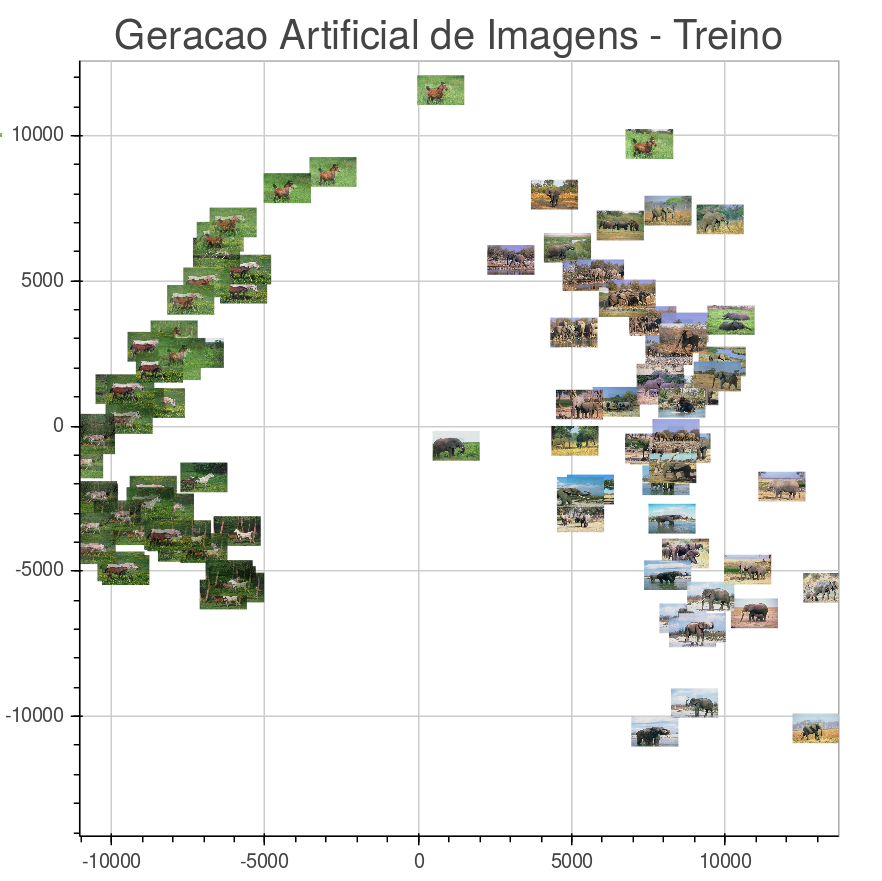
\includegraphics[width=.7\linewidth]{\detokenize{figuras/visualizacao/vis-images.png}}
    \end{center}
  \caption[Visualização do impacto do método de extração de características na separação entre classes. Possível verificar que o BIC utiliza as intensidades como principal representação de uma imagem.]{Visualização do impacto do método de extração de características na separação entre classes. Possível verificar que o BIC utiliza as intensidades como principal representação de uma imagem. \textit{Fonte:~Elaborado pela autora.}}
  \label{fig:vis_images}
\end{figure}

%-------------------------------------------------------------------------------
\subsubsection{Resultados}

Para análise estatística, todas as combinações de conversão para escala de cinza e métodos de extração de características foram testados. A combinação \emph{Gleam} e \emph{ACC} obteve o melhor \textit{F1-Score} para as classes \emph{Elevante} e \emph{Cavalo}. O \textit{boxplot} apresentado na Figura \ref{fig:resultados:1:melhor} retrata a média dos \textit{F1-Scores} das 40 combinações deste experimento. A Tabela \ref{fig:resultados:1:tabmelhor} mostra os valores de tal métrica para o cálculo dos testes estatísticos. Como pode ser observado, o método de \emph{composição}, exemplificado na Figura \ref{fig:resultados:1:mistura}, obteve o melhor \textit{F1-Score}. Como reportado anteriormente para o método BIC, a melhor geração para essas classes é o método de mistura. Interessante notar que, a preferência pelo método de geração parece estar relacionada ao método de extração. Isso se deve, possivelmente, pelo fato de o melhor método de extração indicar as características mais relevantes das imagens.


\begin{figure}[!htbp]
  \begin{center}
      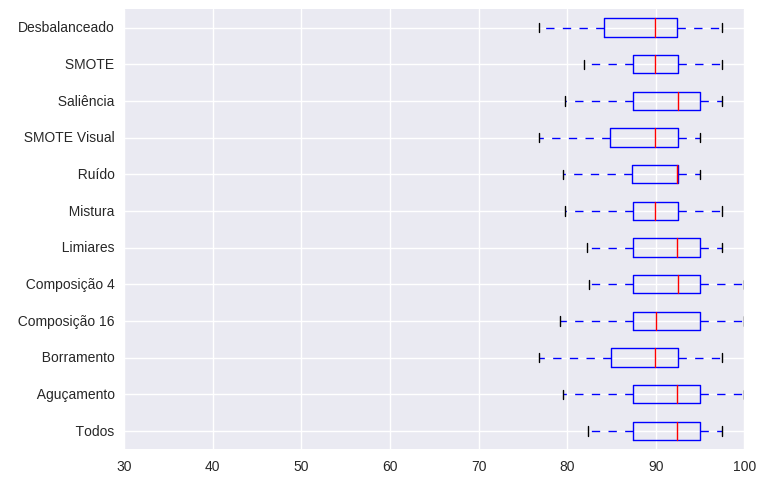
\includegraphics[width=0.8\linewidth]{\detokenize{figuras/resultados/1/ACC_Gleam_elefante-cavalo.png}}
  \end{center}
  \caption[Conversão em escala de cinza com Gleam e ACC como método de extração de características. Nota-se que o método de geração baseado em Composição 4 obteve maior valor de \textit{F1-Score}.]{Conversão em escala de cinza com Gleam e ACC como método de extração de características. Nota-se que o método de geração baseado em Composição 4 obteve maior valor de \textit{F1-Score}. \textit{Fonte:~Elaborado pela autora.}}
  \label{fig:resultados:1:melhor}
\end{figure}

\begin{table}[!htbp]
\begin{center}
\caption{Resultados de \textit{F1-score} para as classes \emph{Cavalo} e \emph{Elefante}, utilizando \emph{Gleam} como método para conversão em escala de cinza e \emph{ACC} para extração de características. Nota-se que o método de geração baseado em Composição 4 obteve maior valor de \textit{F1-Score}.}
\label{fig:resultados:1:tabmelhor}
\begin{tabular}{|l|c|c|}
\hline
\textbf{Gleam \& ACC} & \textbf{Média}     & \textbf{Desvio Padrão} \\ \hline
Todos                 & 91.090913          & 4.559066               \\ \hline
Aguçamento            & 91.002678          & 4.907016               \\ \hline
Borramento            & 89.394500          & 5.103498               \\ \hline
Composição 16         & 90.934305          & 4.399334               \\ \hline
Composição 4          & \textbf{91.773528} & 4.909852               \\ \hline
Limiares              & 90.893133          & 5.285833               \\ \hline
Mistura               & 90.177055          & 4.409787               \\ \hline
Ruído                 & 89.337770          & 5.169757               \\ \hline
SMOTE Visual          & 88.616535          & 5.567976               \\ \hline
Saliência             & 91.282655          & 4.230281               \\ \hline
SMOTE                 & 90.173808          & 4.566863               \\ \hline
Desbalanceado         & 88.258567          & 5.538461               \\ \hline
\end{tabular}
\end{center}
\end{table}

\begin{figure}[!htbp]
    \begin{center}
    \subfloat[Composição]{
      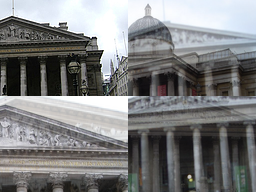
\includegraphics[width=.5\linewidth]{\detokenize{figuras/resultados/1/resultado-composicao.png}}
    }
   \caption[Geração artificial com o método \emph{composição} com quatro imagens da classe \textit{Elefante}.]{Geração artificial com o método \emph{composição} com quatro imagens da classe \textit{Elefante}. \textit{Fonte:~Elaborado pela autora.}}
   \label{fig:resultados:1:mistura}
\end{center}
\end{figure}

Considerando a análise da melhor combinação dos métodos de representação da imagem, foi verificado também a performance dos rebalanceamentos em um cenário mais complexo: o de maior variância dos \textit{F1-Scores}, dadas as 40 combinações da validação. A Figura \ref{fig:resultados:1:pior} mostra o gráfico de \textit{boxplot} referente aos resultados da Tabela \ref{fig:resultados:1:tabpior}. O melhor método de rebalanceamento para tal cenário foi o de geração artificial de imagens de adição de \emph{ruído}, exemplificado na Figura \ref{fig:resultados:1:ruido}. Referente aos resultados da Tabela~\ref{fig:resultados:1:tabpior}, o par de métodos \emph{MSB} e \emph{HOG} obteve maior valor de variância -- para conversão de escala de cinza e extração de características, respectivamente.

\begin{figure}[!htbp]
    \begin{center}
      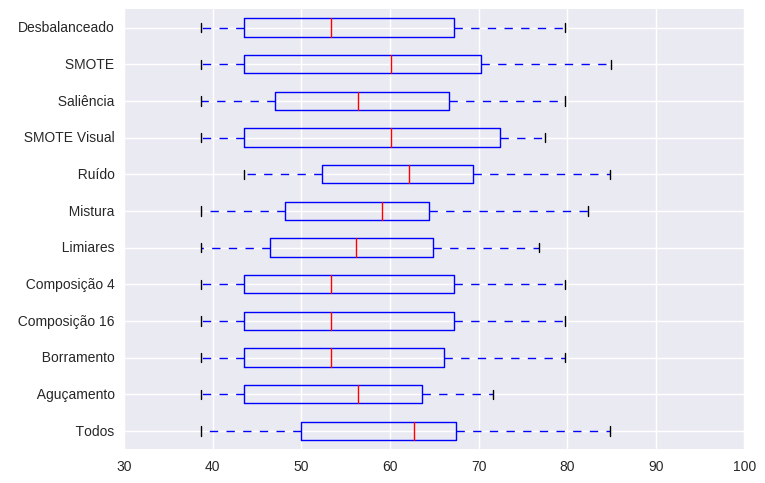
\includegraphics[width=0.8\linewidth]{\detokenize{figuras/resultados/1/HOG_MSB_elefante-cavalo.png}}
    \end{center}
    \caption[Conversão em escala de cinza com MSB e HOG como método de extração de características. Essa combinação de métodos obteve a maior variância de \textit{F1-Score}. Nota-se que o método de geração de ruído apresentou-se como o melhor.]{Conversão em escala de cinza com MSB e HOG como método de extração de características.  Essa combinação de métodos obteve a maior variância de \textit{F1-Score}. Nota-se que a geração de ruído apresentou-se como o melhor método. \textit{Fonte:~Elaborado pela autora.}}
    \label{fig:resultados:1:pior}
\end{figure}

\begin{table}[!htbp]
\begin{center}
\caption{Resultados de \textit{F1-Score} para as classes \emph{Cavalo} e \emph{Elefante}, utilizando MSB como método para conversão em escala de cinza e \emph{HOG} para extração de características. O método de adição de ruído foi aquele que obteve melhor valor de \textit{F1-Score}.}
\label{fig:resultados:1:tabpior}
\begin{tabular}{|l|c|c|}
\hline
\textbf{MSB \& HOG} & \textbf{Média}     & \textbf{Desvio Padrão} \\ \hline
Todos               & 60.000127          & 12.063967              \\ \hline
Aguçamento          & 54.809555          & 10.610213              \\ \hline
Borramento          & 55.588173          & 13.275734              \\ \hline
Composição 16       & 55.667145          & 13.341421              \\ \hline
Composição 4        & 55.652205          & 13.323408              \\ \hline
Limiares            & 55.652268          & 11.547820              \\ \hline
Mistura             & 57.826535          & 10.882912              \\ \hline
Ruído               & \textbf{62.174910} & 10.746760              \\ \hline
SMOTE Visual        & 58.920085          & 14.765860              \\ \hline
Saliência           & 56.322367          & 12.169296              \\ \hline
SMOTE               & 58.342450          & 13.768688              \\ \hline
Desbalanceado       & 55.667145          & 13.341421              \\ \hline
\end{tabular}
\end{center}
\end{table}

\begin{figure}[!htbp]
  \begin{center}
    \subfloat[Original]{
      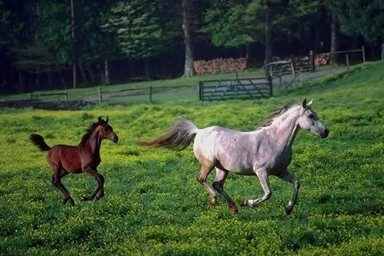
\includegraphics[width=.5\linewidth]{\detokenize{figuras/resultados/1/original-ruido.png}}
    }
    \subfloat[Ruído]{
      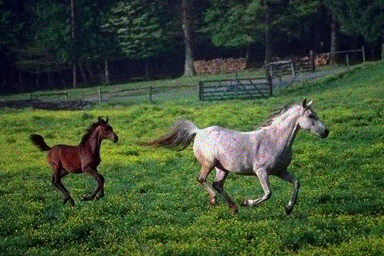
\includegraphics[width=.5\linewidth]{\detokenize{figuras/resultados/1/resultado-ruido.png}}
    }
 \caption[Imagem gerada utilizando \emph{adição de ruído} em imagens da classe \emph{Cavalo}]{Imagem gerada utilizando \emph{adição de ruído} em imagens da classe \emph{Cavalo}. \textit{Fonte:~Elaborado pela autora.}}
 \label{fig:resultados:1:ruido}
 \end{center}
\end{figure}

%-------------------------------------------------------------------------------
\FloatBarrier
\subsubsection{Discussão}

% Tukey HSD Post-hoc Test...
% Group 1 vs Group 2: Diff=1.9152, 95%CI=-0.7500 to 4.5805, p=0.2073
% Group 1 vs Group 3: Diff=3.5150, 95%CI=0.8497 to 6.1802, p=0.0062
% Group 2 vs Group 3: Diff=1.5997, 95%CI=-1.0656 to 4.2650, p=0.3315

Para o resultado da combinação dos melhores métodos de conversão em escala de cinza e extração de características, o teste \textit{post-hoc} HSD de Tukey revelou que não há diferença estatística entre a base desbalanceada e o SMOTE ($\textit{p-value} = 0.2073$). Porém, indicou que existe uma significância entre o desbalanceamento e a geração artificial ($\textit{p-value} = 0.0062$). Isso significa que o melhor método para rebalancear essas classes é a geração artificial utilizando o método de misturas de duas imagens. Ainda de acordo com o teste, não há evidência estatística da relevância do resultado da combinação de maior variância. Portanto, todos os próximos experimentos relatam apenas os resultados da melhor combinação.

%%%%%%%%%%%%%%%%%%%%%%%%%%%%%%%%%%%%%%%%%%%%%%%%%%%%%%%%%%%%%%%%%%%%%%%%%%%%%%%%
\subsection{Experimento 2: duas classes de difícil diferenciação}

O experimento anterior considerou classes relativamente distintas. Por isso, classes de difícil diferenciação também foram testadas e são reportadas a seguir.

\subsubsection{Protocolo}
\begin{enumerate}
\item \textbf{Classes de imagens originais}: \textit{Praia} e \emph{Montanha} foram escolhidas por serem as classes que possuem maior dificuldade de diferenciação da base Corel~\cite{Wang2001}. Apresentam alta taxa de sobreposição de intensidades de cores e texturas, conforme testes realizados. Uma imagem de exemplo de cada classe é apresentada na Figura~\ref{fig:resultados:2:base}.

\begin{minipage}{\linewidth}
\begin{figure}[H]
  \begin{center}
    \subfloat[Montanha]{
      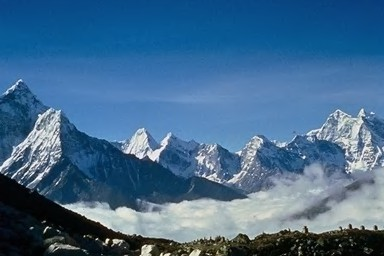
\includegraphics[width=.48\linewidth]{\detokenize{figuras/resultados/2/montanha.png}}
    }
    \subfloat[Praia]{
      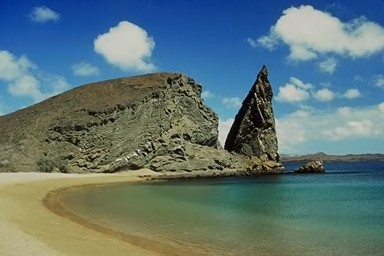
\includegraphics[width=.48\linewidth]{\detokenize{figuras/resultados/2/praia.png}}
    }
    \caption[Imagens representativas das classes \textit{Praia} e \textit{Montanha} da base de imagens Corel.]{Imagens representativas das classes \textit{Praia} e \textit{Montanha} da base de imagens Corel. \textit{Fonte:~Elaborado pela autora.}}
    \label{fig:resultados:2:base}
\end{center}
\end{figure}
\end{minipage}

\item \textbf{Desbalanceamento}: as duas classes contém 100 imagens cada, portanto são balanceadas. Para esse experimento, foram utilizadas as 40 combinações de desbalanceamento dos $k=5$ folds.

\item \textbf{Método para geração artificial}: todos os métodos de geração foram testados. Os que obtiveram melhores resultados foram os métodos de: saliência, aguçamento e a utilização de todos os tipos de gerações aleatórios. A Figura~\ref{fig:resultados:2:saliencia} exemplifica uma geração artificial deste experimento, utilizando o método de \emph{saliência}.

\begin{minipage}{\linewidth}
\begin{figure}[H]
  \begin{center}
    \subfloat[Original]{
      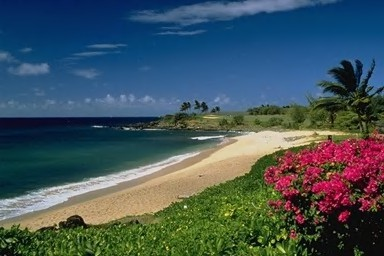
\includegraphics[width=.33\linewidth]{\detokenize{figuras/resultados/2/original-saliencia.png}}
    }
    \subfloat[Original]{
      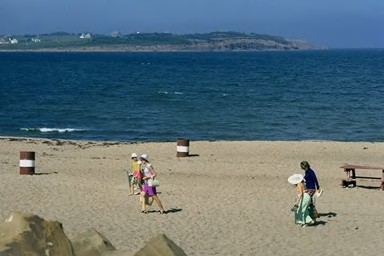
\includegraphics[width=.33\linewidth]{\detokenize{figuras/resultados/2/original2-saliencia.png}}
    }
    \subfloat[Saliência]{
      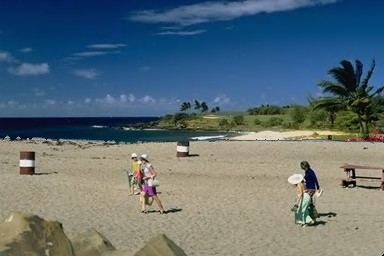
\includegraphics[width=.33\linewidth]{\detokenize{figuras/resultados/2/resultado-saliencia.png}}
    }
 \caption[Geração artificial utilizando o método de \emph{saliência} em duas imagens da classe \emph{Praia} da base de imagens Corel.]{Geração artificial utilizando o método de \emph{saliência} em duas imagens da classe \emph{Praia} da base de imagens Corel. \textit{Fonte:~Elaborado pela autora.}}
 \label{fig:resultados:2:saliencia}
 \end{center}
\end{figure}
\end{minipage}

\item \textbf{Conversão em escala de cinza}: todos os métodos de conversão em escala de cinza foram testados. O método \emph{Luma} resultou em melhor \textit{F1-Score}.

\item \textbf{Extração de características}: todos os métodos para extração foram testados. O método CCV destacou-se como o melhor método para extrair as características que melhor diferenciam essas classes.

\item \textbf{Classificação}: o classificador KNN com $K=1$ foi utilizado.
\end{enumerate}

%-------------------------------------------------------------------------------
\subsubsection{Resultados}

A combinação dos métodos \emph{Luma} e CCV resultou em melhores valores de \textit{F1-Score}. Como pode ser visto na Tabela \ref{tab:resultados:2:melhor}, diversos métodos de geração artificial de imagens obtiveram resultados melhores que o SMOTE, e na sua maioria maiores do que a base desbalanceada. Destacam-se os métodos de saliência, mistura e composição.

%Na Figura \ref{fig:resultados:2:melhor} é possível verificar o \textit{boxplot} dos \textit{F1-Scores} para as classes desbalanceadas, rebalanceadas com SMOTE após a extração de características e rebalanceadas com os métodos de geração artificial como primeiro passo do \textit{pipeline}.

% \begin{figure}[!htbp]
%   \begin{center}
%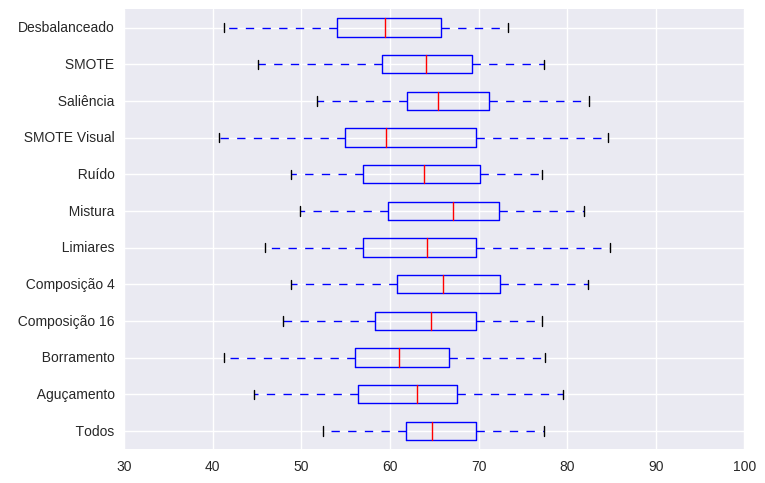
\includegraphics[width=\linewidth]{\detokenize{figuras/resultados/2/BIC_Luminance_praia-montanha.png}}
%   \end{center}
%   \caption[Boxplot das classes \emph{Praia} e \emph{Montanha} para a conversão em escala de cinza com \emph{Luminância'} e BIC como método de extração de características.]{Boxplot das classes \emph{Praia} e \emph{Montanha} para a conversão em escala de cinza com \emph{Luminância'} e BIC como método de extração de características. \textit{Fonte:~Elaborado pela autora.}}
%   \label{fig:resultados:2:melhor}
% \end{figure}

\begin{table}[H]
\begin{center}
\caption{Resultados de \textit{f1-score} para as classes \emph{Praia} e \emph{Montanha}, utilizando \emph{Luma} como método para conversão em escala de cinza e \emph{CCV} para extração de características.}
\label{tab:resultados:2:melhor}
\begin{tabular}{|l|c|c|}
\hline
\textbf{Luma \& CCV} & \textbf{Média}     & \textbf{Desvio Padrão} \\ \hline
   Todos        & \textbf{66.015325} & 5.621643  \\ \hline
  Aguçamento    & \textbf{66.684300} & 5.619944  \\ \hline
  Borramento    & 62.186430 & 6.509084  \\ \hline
  Composição 16 & 63.225965 & 7.920787  \\ \hline
  Composição 4  & 63.824235 & 5.621168  \\ \hline
  Limiares      & 64.453515 & 6.769440  \\ \hline
  Mistura       & 59.506260 & 6.472903  \\ \hline
  Ruído         & 64.202075 & 7.231610  \\ \hline
  SMOTE Visual  & 59.512530 & 7.737273  \\ \hline
  Saliência     & \textbf{66.260870} & 5.732209  \\ \hline
 SMOTE          & 65.531135 & 4.714502  \\ \hline
Desbalanceado   & 59.640090 & 8.675836  \\ \hline
\end{tabular}
\end{center}
\end{table}

% \begin{minipage}{\linewidth}
%   \begin{figure}[H]
%     \subfloat[Original]{
%       \includegraphics[width=.33\linewidth]{\detokenize{figuras/resultados/2/original-mistura.png}}
%     }
%     \subfloat[Original]{
%       \includegraphics[width=.33\linewidth]{\detokenize{figuras/resultados/2/original2-mistura.png}}
%     }
%     \subfloat[Mistura]{
%       \includegraphics[width=.33\linewidth]{\detokenize{figuras/resultados/2/resultado-mistura.png}}
%     }
%     \caption[Geração artificial utilizando o método de \emph{mistura} em duas imagens da classe \emph{Montanha} da base de imagens Corel.]{Geração artificial utilizando o método de \emph{mistura} em duas imagens da classe \emph{Montanha} da base de imagens Corel. \textit{Fonte:~Elaborado pela autora.}}
%     \label{fig:resultados:2:mistura}
%   \end{figure}
% \end{minipage}

%-------------------------------------------------------------------------------
\subsubsection{Discussão}

De acordo com o teste HSD de Tukey realizado, foi encontrado $\textit{p-value} = 0.0003$ na comparação da base desbalanceada com a base rebalanceada utilizando o método SMOTE e $\textit{p-value} = 0.0000$ com a geração artificial. Isso indica que ambos os métodos obtiveram relevância estatística quando comparados ao original. Porém, ao comparar o SMOTE com a geração artificial, o teste resultou em $\textit{p-value} = 0.7122$. Tal valor indica que não há diferença significativa entre os métodos SMOTE e os métodos de geração artificial de imagens.



%%%%%%%%%%%%%%%%%%%%%%%%%%%%%%%%%%%%%%%%%%%%%%%%%%%%%%%%%%%%%%%%%%%%%%%%%%%%%%%%
\FloatBarrier
\subsection{Experimento 3: multiclasses}

Os dois experimentos anteriores analisaram o rebalanceamento de apenas duas classes. Este experimento apresenta a geração artificial de imagens aplicada a três bases multiclasses: Corel, Caltech e Produce. Seus resultados são discutidos individualmente.

\subsubsection{Base de imagens Corel}

\subsubsubsection{Protocolo}

\begin{enumerate}
\item \textbf{Base de imagens originais}: esse experimento foi realizado com a base de imagens Corel-1000, composta por fotografias que representam 10 classes variadas: tribos africanas, praia, construções, ônibus, dinossauros, flores, elefantes, cavalos, montanhas e tipos de comidas \cite{Wang2001}. Para fins de exemplificação, são apresentadas imagens que representam essas classes na Figura \ref{fig:resultados:3:base}.

\begin{minipage}{\linewidth}
\begin{figure}[H]
  \begin{center}
    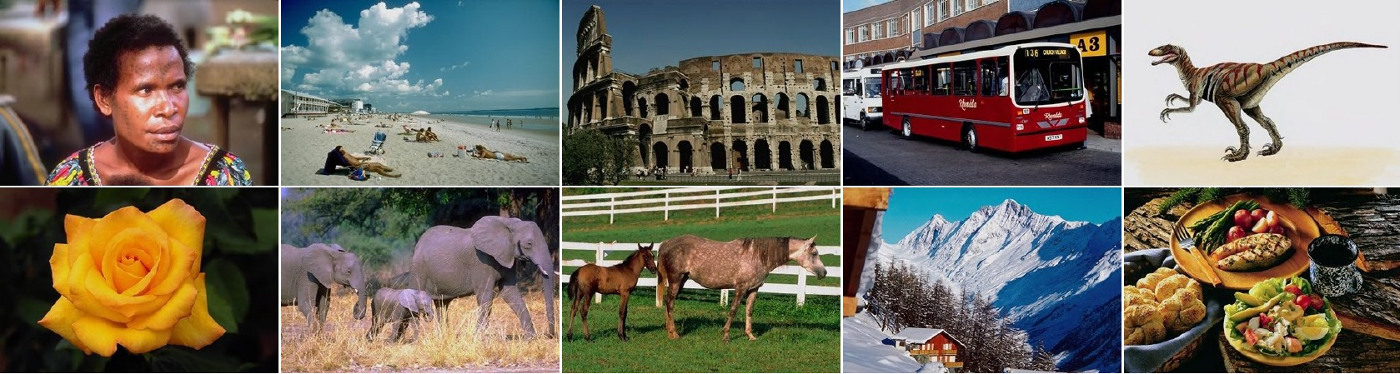
\includegraphics[width=\linewidth]{\detokenize{figuras/quantizacao/fig_COREL_dataset.jpg}}
    \caption[Base de imagens Corel-1000 \cite{Wang2001}. Essa base é composta por fotografias que representam 10 classes variadas: tribos africanas, praia, construções, ônibus, dinossauros, flores, elefantes, cavalos, montanhas e tipos de comidas.]{Base de imagens Corel-1000 \cite{Wang2001}. Essa base é composta por fotografias que representam 10 classes variadas: tribos africanas, praia, construções, ônibus, dinossauros, flores, elefantes, cavalos, montanhas e tipos de comidas. \textit{Fonte:~\cite{Ponti2016}.}}
    \label{fig:resultados:3:base}
\end{center}
\end{figure}
\end{minipage}

\item \textbf{Desbalanceamento}: realizaram-se 200 combinações de desbalanceamento dos 5 \textit{folds} para as 10 classes.

\item \textbf{Método para geração artificial}: o método que atingiu o maior \textit{F1-Score} de geração artificial foi a mistura. Por esse motivo, ela está exemplificada na Figura \ref{fig:resultados:3.1:mistura}.

\begin{minipage}{\linewidth}
\begin{figure}[H]
  \begin{center}
    \subfloat[Original]{
      \includegraphics[width=.33\linewidth]{\detokenize{figuras/resultados/3/original-mistura.png}}
    }
    \subfloat[Original]{
      \includegraphics[width=.33\linewidth]{\detokenize{figuras/resultados/3/original2-mistura.png}}
    }
    \subfloat[Mistura]{
      \includegraphics[width=.33\linewidth]{\detokenize{figuras/resultados/3/resultado-mistura.png}}
    }
    \caption[Geração artificial de mistura para imagens da base Corel \cite{Wang2001}.]{Geração artificial de mistura para imagens da base Corel. \textit{Fonte:~Elaborado pela autora.}}
    \label{fig:resultados:3.1:mistura}
\end{center}
\end{figure}
\end{minipage}

\item \textbf{Conversão em escala de cinza}: todos os métodos foram testados e o método \textit{Gleam} obteve os melhores resultados.

\item \textbf{Extração de características}: dada a combinação de todos os métodos, o LBP se sobressaiu entre eles.

\item \textbf{Classificação}: KNN com $K=1$ foi o classificador utilizado.
\end{enumerate}

%-------------------------------------------------------------------------------
\subsubsubsection{Resultados}

Ao realizar o experimento com as 10 classes da base Corel, a combinação de Gleam para conversão em escala de cinza; e LBP como método de extração de características, resultou em melhores \textit{F1-Scores}. A base Corel é originalmente balanceada, portanto a cada combinação dos \textit{folds}, uma classe era considerada minoritária e três dos seus \textit{folds} eram descartados (restando um para treino e um para teste). Isso permitiu testar a base como desbalanceada. A Tabela \ref{tab:resultados:3.1} mostra a média e o desvio padrão dos \textit{F1-Scores} encontrados nesse experimento. Note que a geração artificial com o método \emph{mistura} obteve \textit{F1-Score} similar ao SMOTE.

\begin{table}[H]
\begin{center}
\caption{Resultados de \textit{F1-Score} para as 10 classes da Corel, utilizando \emph{Gleam} como método para conversão em escala de cinza e \emph{LBP} para extração de características. Note que a geração artificial com o método \emph{mistura} obteve \textit{F1-Score} similar ao SMOTE.}
\label{tab:resultados:3.1}
\begin{tabular}{|l|c|c|}
\hline
\textbf{LBP Gleam} & \textbf{Média}     & \textbf{Desvio Padrão} \\ \hline
   Todos        &  61.216388 &  2.205391  \\ \hline
  Aguçamento    &  61.098384 &  2.275732  \\ \hline
  Borramento    &  60.369376 &  2.254895  \\ \hline
  Composição 16 &  60.630235 &  2.212156  \\ \hline
  Composição 4  &  60.568624 &  2.254904  \\ \hline
  Limiares      &  61.296003 &  2.101686  \\ \hline
  Mistura       &  \textbf{61.366671} &  2.225635  \\ \hline
  Ruído         &  60.825884 &  2.358098  \\ \hline
  SMOTE Visual  &  60.886122 &  2.321783  \\ \hline
  Saliência     &  61.050988 &  2.271443  \\ \hline
 SMOTE          &  \textbf{61.368896} &  2.148675  \\ \hline
Desbalanceado   &  60.362256 &  2.290263  \\ \hline
\end{tabular}
\end{center}
\end{table}

%-------------------------------------------------------------------------------
\subsubsubsection{Discussão}

O rebalanceamento com o método de \emph{mistura} e com o SMOTE tiveram uma performance quase idêntica (i.e. $\textit{p-value} = 0.9948$). Mas apesar de \textit{F1-Scores} também parecerem similares à base desbalanceada, o teste HSD de Tukey confirmou que há diferença estatística significante entre eles ($\textit{p-value} = 0.0000$). Dessa forma, tanto o SMOTE quanto a geração artificial rebalancearam a base satisfatoriamente.

%%%%%%%%%%%%%%%%%%%%%%%%%%%%%%%%%%%%%%%
\subsubsection{Base de imagens Caltech}

\subsubsubsection{Protocolo}

\begin{enumerate}
\item \textbf{Base de imagem original}: foi utilizada a base Caltech101-600 \cite{Fei-Fei2007}. Desta base, foi utilizado um conjunto de seis classes balanceadas: aviões, bonsais, candelabros, tartarugas, motocicletas e relógios. Imagens que representam essas classes são apresentadas na Figura \ref{fig:resultados:3.2:base}.

\begin{minipage}{\linewidth}
\begin{figure}[H]
  \begin{center}
    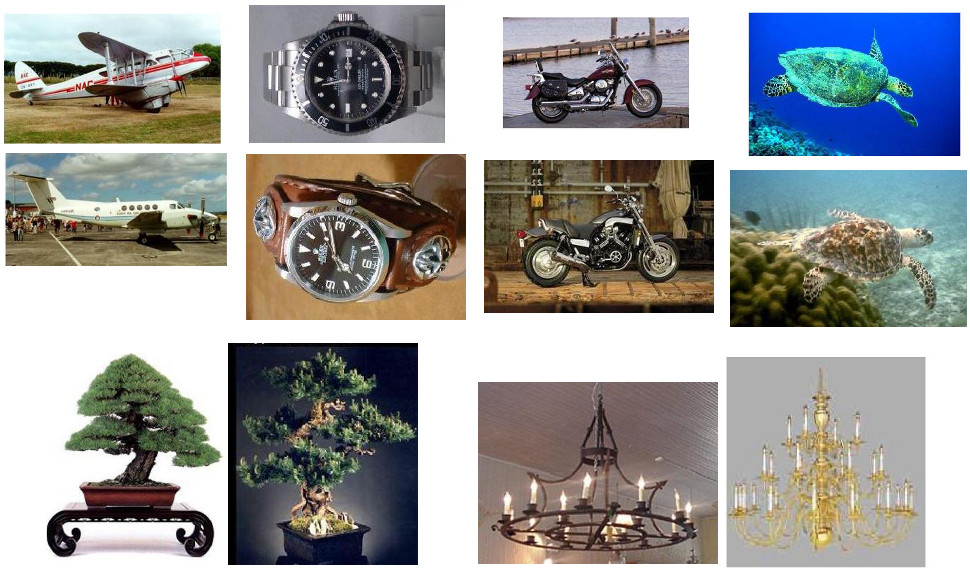
\includegraphics[width=\linewidth]{\detokenize{figuras/quantizacao/fig_Caltech101_dataset.jpg}}
    \caption{Conjunto de seis classes balanceadas: aviões, bonsais, candelabros, tartarugas, motocicletas e relógios da base de imagens Caltech101 \cite{Fei-Fei2007}. \textit{Fonte:~\cite{Ponti2016}.}}
    \label{fig:resultados:3.2:base}
\end{center}
\end{figure}
\end{minipage}

\item \textbf{Desbalanceamento}: 120 combinações de 5 fold para as 6 classes) foram realizadas. Cobrindo, assim, todas as possibilidades para garantir que cada imagem pudesse pertencer a majoritária, minoritária, treino, teste ou não ser utilizada na classificação.
\item \textbf{Método para geração artificial}: o melhor resultado em termos de geração artificial foi utilizando todas as gerações. A Figura   \ref{fig:resultados:3.2:limiares} apresenta um exemplo da geração com mistura de limiares, uma das possíveis gerações artificiais.

\begin{minipage}{\linewidth}
  \begin{figure}[H]
    \begin{center}
    \subfloat[Original]{
      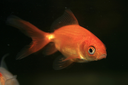
\includegraphics[height=1.7cm,keepaspectratio]{\detokenize{figuras/resultados/3/original-limiares.png}}
    }
    \subfloat[Original]{
      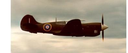
\includegraphics[height=1.7cm,keepaspectratio]{\detokenize{figuras/resultados/3/original2-limiares.png}}
    }
    \subfloat[Mistura limiarizada]{
      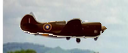
\includegraphics[height=1.7cm,keepaspectratio]{\detokenize{figuras/resultados/3/resultado-limiares.png}}
    }
    \caption[Exemplo de uma geração artificial utilizando o método de combinação de limiares para a base Caltech.]{Exemplo de uma geração artificial utilizando o método de combinação de limiares para a base Caltech. \textit{Fonte:~Elaborado pela autora.}}
    \label{fig:resultados:3.2:limiares}
  \end{center}
  \end{figure}
\end{minipage}

\item \textbf{Conversão em escala de cinza}: todos os métodos foram testados. O que obteve melhores resultados foi o \textit{Intensity'}.
\item \textbf{Extração de características}: de todos os métodos foram testados, o HOG foi o melhor método de extração de características.
\item \textbf{Classificação}: classificador KNN com $K=1$.
\end{enumerate}

%-------------------------------------------------------------------------------
\subsubsubsection{Resultados}

Considerando que essa base possui 6 classes, 120 sub-experimentos foram necessários para cobrir todas as possibilidades de desbalanceamento. Os resultados de tais experimentos são apresentados na Tabela \ref{tab:resultados:3.2}. É possível notar que tanto o SMOTE quanto a geração artificial utilizando todos os métodos obtiveram um \textit{F1-Score} melhor que a versão desbalanceada. Interessante notar que a combinação aleatória uniforme de todos os métodos obteve um \textit{F1-Score} melhor do que cada método individualmente.

\begin{table}[H]
\begin{center}
\caption{Resultados do experimento com a base Caltech. É possível notar que tanto o SMOTE quanto a geração artificial utilizando todos os métodos obtiveram um \textit{F1-Score} melhor que a versão desbalanceada.}
\label{tab:resultados:3.2}
\begin{tabular}{|l|c|c|}
\hline
\textbf{HOG Intensity'} & \textbf{Média}     & \textbf{Desvio Padrão} \\ \hline
   Todos        &  \textbf{77.591493} &  3.387543  \\ \hline
  Aguçamento    &  76.982412 &  3.482750  \\ \hline
  Borramento    &  75.736587 &  3.812333  \\ \hline
  Composição 16 &  75.742438 &  3.823391  \\ \hline
  Composição 4  &  75.787022 &  3.794589  \\ \hline
  Limiares      &  76.785628 &  3.652596  \\ \hline
  Mistura       &  77.186702 &  3.382386  \\ \hline
  Ruído         &  77.344959 &  3.664212  \\ \hline
  SMOTE Visual  &  75.486170 &  4.405685  \\ \hline
  Saliência     &  76.587268 &  3.600158  \\ \hline
 SMOTE          &  \textbf{77.755417} &  3.529355  \\ \hline
Desbalanceado   &  75.732382 &  3.833682  \\ \hline
\end{tabular}
\end{center}
\end{table}

%-------------------------------------------------------------------------------
\subsubsubsection{Discussão}

Com o teste \textit{post-hoc} HSD de Tukey ficou comprovada a suposição de que os resultados do SMOTE e da geração artificial utilizando todos os métodos não possuem diferença estatística. Isso porque resultaram em $\textit{p-value} = 0.9333$. Porém, entre o desbalanceado e o SMOTE ou a geração obteve-se $\textit{p-value} < 0.000$. O que indica que todos os métodos de rebalanceamento foram satisfatórios para a base Caltech.

% Desbalanceado vs SMOTE: Diff=2.0230, 95%CI=0.9330 to 3.1131, \textit{p-value} =0.0000
% Desbalanceado vs Geração artificial: Diff=1.8591, 95%CI=0.7691 to 2.9491, \textit{p-value} =0.0002
% SMOTE vs Geração artificial: Diff=-0.1639, 95%CI=-1.2540 to 0.9261, \textit{p-value} =0.9333


%%%%%%%%%%%%%%%%%%%%%%%%%%%%%%%%%%%%%%%
\subsubsection{Base de imagens Produce}

\subsubsubsection{Protocolo}

\begin{enumerate}
\item \textbf{Base de imagens originais}: Produce, composta por imagens de vegetais e frutas tropicais \cite{Rocha2010}. Posuem fundo similar mas muitas mudanças na iluminação, no número de objetos e na escala. Amostras das imagens dessa base são apresentadas na Figura \ref{fig:resultados:3.3:base}. Essa base contem 14 classes e um total de 1400 imagens.

\begin{minipage}{\linewidth}
\begin{figure}[H]
  \begin{center}
    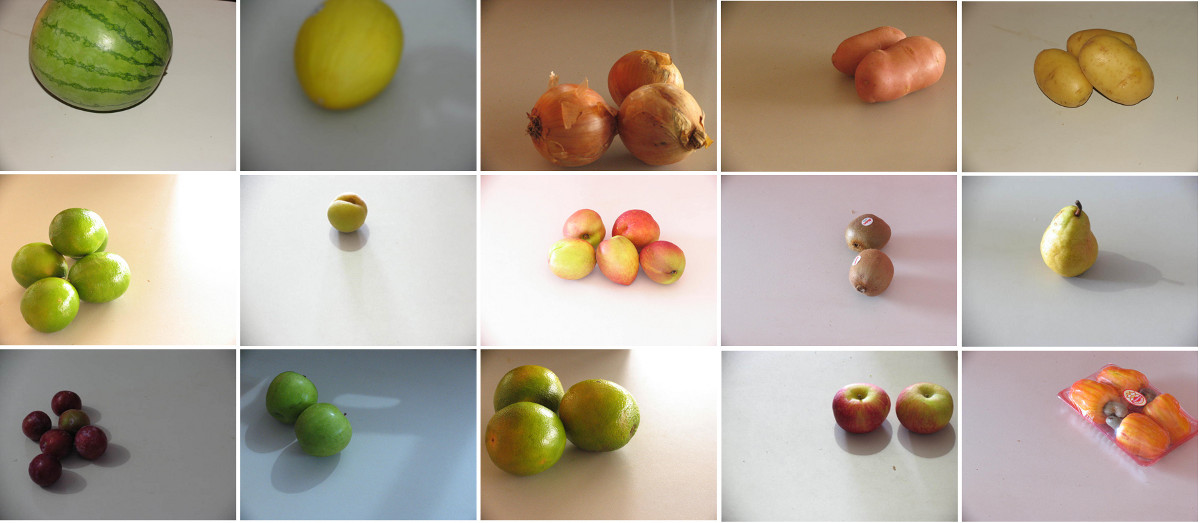
\includegraphics[width=\linewidth]{\detokenize{figuras/quantizacao/fig_Produce_dataset.jpg}}
    \caption{Base de imagens \textit{Produce}, composta por imagens de vegetais e frutas tropicais \cite{Rocha2010}. \textit{Fonte:~\cite{Ponti2016}.}}
    \label{fig:resultados:3.3:base}
\end{center}
\end{figure}
\end{minipage}

\item \textbf{Desbalanceamento}: considerando que a base Produce é balanceada, 280 combinações dos 5 \textit{folds} das 14 classes foram testadas. Dessa forma todas as classes tiveram chance de serem a classe minoritária e, assim, rebalanceadas.
\item \textbf{Método para geração artificial}: o melhor método de geração para a classe Produce foi a \emph{mistura}, exemplificada na Figura \ref{fig:resultados:3.3:mistura}.

\begin{minipage}{\linewidth}
  \begin{figure}[H]
    \begin{center}
    \subfloat[Original]{
      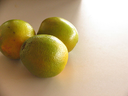
\includegraphics[width=.32\linewidth]{\detokenize{figuras/resultados/3/original-mistura-produce.png}}
    }
    \subfloat[Original]{
      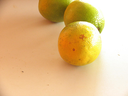
\includegraphics[width=.32\linewidth]{\detokenize{figuras/resultados/3/original2-mistura-produce.png}}
    }
    \subfloat[Mistura]{
      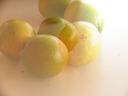
\includegraphics[width=.32\linewidth]{\detokenize{figuras/resultados/3/resultado-mistura-produce.png}}
    }
    \caption[Exemplo de geração artificial utilizando a \emph{mistura} de duas imagens para a classe \textit{Produce}.]{Exemplo de geração artificial utilizando a mistura de duas imagens para a classe \textit{Produce}. \textit{Fonte:~Elaborado pela autora.}}
    \label{fig:resultados:3.3:mistura}
    \end{center}
  \end{figure}
\end{minipage}

\item \textbf{Conversão em escala de cinza}: todas as combinações de métodos foram testadas. \emph{Luma} destacou-se como o melhor método para converter a imagem em escala de cinza.
\item \textbf{Extração de características}: todos os métodos foram testados. O LBP obteve os melhores resultados.
\item \textbf{Classificação}: classificador KNN com $K=1$.
\end{enumerate}

%-------------------------------------------------------------------------------
\subsubsubsection{Resultados}

A Tabela \ref{tab:resultados:3.3} apresenta a média e o desvio padrão dos \textit{F1-Scores} encontrados nos 280 sub-experimentos para a classe Produce. Esses cobrem todas as possibilidades de desbalanceamento. O método de \emph{mistura} resultou no melhor \textit{F1-Score}.

\begin{table}[H]
\begin{center}
\caption{Resultados de \textit{F1-Scores} para a base de imagens \textit{Produce}. O método \emph{mistura} apresentou-se como o melhor.}
\label{tab:resultados:3.3}
\begin{tabular}{|l|c|c|}
\hline
\textbf{LBP Luma} & \textbf{Média}     & \textbf{Desvio Padrão} \\ \hline
   Todos        &  91.682606 &  1.985052  \\ \hline
  Aguçamento    &  91.463371 &  2.039631  \\ \hline
  Borramento    &  91.493838 &  2.022884  \\ \hline
  Composição 16 &  91.476496 &  2.037559  \\ \hline
  Composição 4  &  91.478369 &  2.021889  \\ \hline
  Limiares      &  91.843197 &  1.934367  \\ \hline
  Mistura       &  \textbf{91.985465} &  1.949951  \\ \hline
  Ruído         &  91.489904 &  2.028988  \\ \hline
  SMOTE Visual  &  91.473853 &  2.031678  \\ \hline
  Saliência     &  91.772214 &  2.006734  \\ \hline
 SMOTE          &  91.869133 &  1.952464  \\ \hline
Desbalanceado   &  91.489904 &  2.028988  \\ \hline
\end{tabular}
\end{center}
\end{table}

%-------------------------------------------------------------------------------
\subsubsubsection{Discussão}

O teste \textit{post-hoc} HSD de Tukey indicou que há relevância estatística entre os \textit{F1-Scores} da base desbalanceada quando comparada com o rebalanceamento utilizando o método de mistura ($ \textit{p-value} = 0.0087$). Mas comparado com SMOTE, o $\textit{p-value} = 0.0607$ indica que não há diferença significante entre ele e a versão original. Ainda assim, o teste resultou em $\textit{p-value} = 0.7658$ para a comparação entre o SMOTE e a geração artificial, indicando que não há significância entre os dois. De qualquer forma, tais resultados indicam que a geração artificial de \emph{mistura} obteve resultado significativo.

\meutodo{O ANOVA foi calculado com os 3 resultados, mas se utilizar só SMOTE e a geração dá p=0.4808 (significante) ao invés de 0.7658 (não significante). O que isso significa?}

%%%%%%%%%%%%%%%%%%%%%%%%%%%%%%%%%%%%%%%%%%%%%%%%%%%%%%%%%%%%%%%%%%%%%%%%%%%%%%%%
\FloatBarrier
\subsection{Experimento 4: classes naturalmente desbalanceadas}

Os experimentos anteriores foram realizados em bases já balanceadas, com o desbalancemento sendo provocado. Este experimento utiliza duas combinações de classes de imagens naturalmente desbalanceadas.

% Os sub-experimentos foram realizados de forma diferente que os anteriores. Isso foi realizado indicando que o número de imagens faltantes são do \textit{fold} que não seria utilizado, caso fosse o caso de bases balanceadas (experimentos anteriores). Ou seja, todas as classes ainda continuam com \textit{5-folds} cada.

\subsubsection{Duas classes}

Esse experimento aponta os resultados para duas classes naturalmente desbalanceadas.

\subsubsubsection{Protocolo}

\begin{enumerate}
\item \textbf{Classes de imagens originais}: as classes utilizadas para esse experimento foram \textit{Eiffel Tower} com 1607 imagens, e \textit{Rome antica} com apenas 125 imagens \cite{Hu2013}.

\begin{minipage}{\linewidth}
\begin{figure}[H]
  \begin{center}
    \subfloat[\textit{Eiffel Tower}]{
      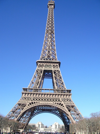
\includegraphics[height=5cm,keepaspectratio]{\detokenize{figuras/resultados/4/class13-1.png}}
    }
    \subfloat[\textit{Rome antica}]{
      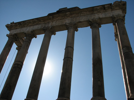
\includegraphics[height=5cm,keepaspectratio]{\detokenize{figuras/resultados/4/class41-2.png}}
    }
    \caption[Imagens das classes \textit{Eiffel Tower} e \textit{Rome antica}.]{Imagens das classes \textit{Eiffel Tower} e \textit{Rome antica}. \textit{Fonte:~Elaborado pela autora.}}
    \label{fig:resultados:4.1:base}
\end{center}
\end{figure}
\end{minipage}

\item \textbf{Desbalanceamento}: natural da base. A classe minoritária é a \textit{Rome antica} com 125 imagens. Dessa forma, a cada combinação dos \textit{folds}, $1607 - 125 = 1482$ imagens foram geradas para rebalancear a base.
\item \textbf{Método para geração artificial}: todas as gerações foram testadas, a que obteve melhor resultado foi a mistura. Essa geração está exemplificada na Figura \ref{fig:resultados:4.1:geracao}.

\begin{minipage}{\linewidth}
  \begin{figure}[H]
    \begin{center}
    \subfloat[Original]{
      \includegraphics[height=3.5cm,keepaspectratio]{\detokenize{figuras/resultados/4/original-mistura.png}}
    }
    \subfloat[Original]{
      \includegraphics[height=3.5cm,keepaspectratio]{\detokenize{figuras/resultados/4/original2-mistura.png}}
    }
    \subfloat[Mistura]{
      \includegraphics[height=3.5cm,keepaspectratio]{\detokenize{figuras/resultados/4/resultado-mistura.png}}
    }
    \caption[Exemplo de geração artificial utilizando a mistura de duas imagens para a classe \textit{Produce}.]{Exemplo de geração artificial utilizando a mistura de duas imagens para a classe \textit{Produce}. \textit{Fonte:~Elaborado pela autora.}}
    \label{fig:resultados:4.1:geracao}
    \end{center}
  \end{figure}
\end{minipage}

\item \textbf{Conversão em escala de cinza}: todos os métodos foram testados. O que obteve melhor \textit{F1-Score} foi o MSB.
\item \textbf{Extração de características}: todos os métodos para extração foram testados. Porém, HOG foi o melhor método para tal.
\item \textbf{Classificação}: KNN com $K=1$.
\end{enumerate}

%-------------------------------------------------------------------------------
\subsubsubsection{Resultados}

O rebalanceamento foi realizado de forma a balancear a classe minoritária \textit{Rome antica}. A Tabela \ref{tab:resultados:4.1} apresenta os resultados de tal rebalanceamento. Nela estão os resultados de média e desvio padrão do rebalanceamento realizado com a combinação dos \textit{folds} das duas classes. O método que obteve maior valor de \textit{F1-Score} foi o de geração artificial com o método de \emph{mistura} de duas imagens.

\begin{table}[H]
\begin{center}
\caption{Resultados de \textit{F1-Score} para as classes \textit{Eiffel Tower} e \textit{Rome antica}, naturalmente desbalanceadas.}
\label{tab:resultados:4.1}
\begin{tabular}{|l|c|c|}
\hline
\textbf{HOG MSB} & \textbf{Média}     & \textbf{Desvio Padrão} \\ \hline
   Todos        &  88.616130 &  1.952745  \\ \hline
  Aguçamento    &  98.345625 &  1.755180  \\ \hline
  Borramento    &  97.173480 &  2.760269  \\ \hline
  Composição 16 &  97.206953 &  2.712589  \\ \hline
  Composição 4  &  97.301088 &  2.381761  \\ \hline
  Limiares      &  98.628050 &  1.142830  \\ \hline
  Mistura       &  \textbf{99.112148} &  0.837440  \\ \hline
  Ruído         &  91.499965 &  1.762218  \\ \hline
  SMOTE Visual  &  82.963755 &  2.678785  \\ \hline
  Saliência     &  98.246915 &  1.526565  \\ \hline
 SMOTE          &  98.471765 &  0.788747  \\ \hline
Desbalanceado   &  97.173480 &  2.760269  \\ \hline
\end{tabular}
\end{center}
\end{table}

%-------------------------------------------------------------------------------
\subsubsubsection{Discussão}

% Tukey HSD Post-hoc Test...
% Desbalanceado vs SMOTE: Diff=1.2983, 95%CI=0.3818 to 2.2147, \textit{p-value} =0.0030
% Desbalanceado vs Geração artificial: Diff=1.9387, 95%CI=1.0222 to 2.8551, \textit{p-value} =0.0000
% SMOTE vs Geração artificial: Diff=0.6404, 95%CI=-0.2761 to 1.5568, \textit{p-value} =0.2255

Apesar de valores de \textit{F1-Score} próximos, de acordo com o teste \textit{post-hoc} de Tukey, foi encontrado $\textit{p-value} = 0.0030$ para a base desbalanceada quando comparado com o rebalanceamento com SMOTE. Isso indica que há significância estatística relevante entre eles. O teste também indicou que há significância entre a base desbalanceada e ela rebalanceada com a geração artificial ($\textit{p-value} = 0.0000$). Porém, se comparados o SMOTE e a geração artificial temos $\textit{p-value} = 0.2255$, indicando que não há diferença significante.

\subsubsection{Multiclasses}
Esse experimento aponta os resultados para três classes naturalmente desbalanceadas.

\subsubsubsection{Protocolo}
\begin{enumerate}

\item \textbf{Classes de imagens originais}: foram utilizadas \textit{Trafalgar Square}, \textit{Madeleine Church} e \textit{Pantheon} \cite{Hu2013}. Essas classes são apresentadas na Figura \ref{fig:resultados:4.2:base}. Vale notar que algumas imagens são muito parecidas (difícil classificação), mas as classes também contêm imagens bem divergentes (fácil diferenciação).

\begin{minipage}{\linewidth}
\begin{figure}[H]
  \begin{center}
    \subfloat[Trafalgar Square]{
      \includegraphics[height=3.5cm,keepaspectratio]{\detokenize{figuras/resultados/4/trafalgar.png}}
    }
    \subfloat[Madeleine Church]{
      \includegraphics[height=3.5cm,keepaspectratio]{\detokenize{figuras/resultados/4/madeleine.png}}
    }
    \subfloat[Pantheon]{
      \includegraphics[height=3.5cm,keepaspectratio]{\detokenize{figuras/resultados/4/pantheon.png}}
    }
    \caption[Imagens exemplo das classes \textit{Trafalgar Square}, \textit{Madeleine Church} e \textit{Pantheon}.]{Imagens exemplo das classes \textit{Trafalgar Square}, \textit{Madeleine Church} e \textit{Pantheon}. \textit{Fonte:~\cite{Hu2013}.}}
    \label{fig:resultados:4.2:base}
\end{center}
\end{figure}
\end{minipage}

\item \textbf{Desbalanceamento}: natural da base. A classe \textit{Trafalgar Square} contém 132 imagens, a \textit{Madeleine Church} 316 e a \textit{Pantheon} 23. Assim, para rebalancear, foram necessários gerar $316 - 132 = 147$ imagens para a \textit{Trafalgar Square} e $316 - 23 = 234$ para a classe \textit{Pantheon}.

\item \textbf{Método para geração artificial}: todas as gerações foram testadas, mas a melhor foi a de composição de quatro imagens, retratada na Figura \ref{fig:resultados:4.2:geracao}.

\begin{figure}[!htbp]
  \begin{center}
  \subfloat{
    \includegraphics[width=.5\linewidth]{\detokenize{figuras/resultados/4/resultado-composicao.png}}
  }
  \caption[Exemplo de geração artificial realizada com a composição de quatro imagens para a classe \textit{Pantheon}.]{Exemplo de geração artificial realizada com a composição de quatro imagens para a classe \textit{Pantheon}. \textit{Fonte:~Elaborado pela autora.}}
  \label{fig:resultados:4.2:geracao}
  \end{center}
\end{figure}

\item \textbf{Conversão em escala de cinza}: de todos os métodos foram testados, o melhor para essas imagens foi o Gleam.
\item \textbf{Extração de características}: todos os métodos para extração foram testados, mas o HOG obteve melhores resultados.
\item \textbf{Classificação}: KNN com $K=1$ foi o classificador utilizado.
\end{enumerate}

%-------------------------------------------------------------------------------
\subsubsubsection{Resultados}

A combinação de melhores métodos para extração e conversão em escala de cinza foram HOG e Gleam, respectivamente. O método de geração artificial de imagens que obteve o melhor \textit{F1-Score} foi a composição de quatro imagens e a Tabela \ref{tab:resultados:4.2} apresenta tais resultados. O método SMOTE piorou significativamente a classificação, mas a geração artificial ficou muito similar a classificação sem gerar imagem nenhuma.

\begin{table}[H]
\begin{center}
\caption{}
\label{tab:resultados:4.2}
\begin{tabular}{|l|c|c|}
\hline
\textbf{HOG Gleam} & \textbf{Média}     & \textbf{Desvio Padrão} \\ \hline
   Todos        &  57.285167 &  6.383771  \\ \hline
  Aguçamento    &  69.726448 &  8.069939  \\ \hline
  Borramento    &  70.621480 &  8.314352  \\ \hline
  Composição 16 &  70.478478 &  8.366100  \\ \hline
  Composição 4  &  \textbf{70.837125} &  7.811876  \\ \hline
  Limiares      &  67.965067 &  5.699239  \\ \hline
  Mistura       &  65.644708 &  6.112751  \\ \hline
  Ruído         &  60.777810 &  8.257640  \\ \hline
  SMOTE Visual  &  53.912270 &  7.907406  \\ \hline
  Saliência     &  67.584110 &  6.236710  \\ \hline
 SMOTE          &  62.322870 &  5.726037  \\ \hline
Desbalanceado   &  70.621480 &  8.314352  \\ \hline
\end{tabular}
\end{center}
\end{table}

%-------------------------------------------------------------------------------
\subsubsubsection{Discussão}
% Tukey HSD Post-hoc Test...
% Desbalanceado vs SMOTE: Diff=-8.2986, 95%CI=-11.4785 to -5.1187, \textit{p-value} =0.0000
% Desbalanceado vs Geração artificial: Diff=0.2156, 95%CI=-2.9643 to 3.3956, \textit{p-value} =0.9858
% SMOTE vs Geração artificial: Diff=8.5143, 95%CI=5.3343 to 11.6942, \textit{p-value} =0.0000

Utilizando o teste \textit{post-hoc} de Tukey, foi encontrado $\textit{p-value} = 0.0000$ para a base desbalanceada versus o rebalanceamento com SMOTE. Isso indica que há significância estatística relevante entre eles. O teste também indicou que não há significância entre a base desbalanceada e ela rebalanceada com a geração artificial ($\textit{p-value} = 0.9858$). Além disso, se comparados o SMOTE e a geração artificial temos $\textit{p-value} = 0.0000$, indicando que há diferença significante. Ou seja, o método SMOTE foi significativamente pior que a base original e o método de geração artificial teve uma melhora não estatisticamente significativa.

%%%%%%%%%%%%%%%%%%%%%%%%%%%%%%%%%%%%%%%%%%%%%%%%%%%%%%%%%%%%%%%%%%%%%%%%%%%%%%%%
\FloatBarrier
\subsection{Experimento 5: classes com muitas imagens}

Por fim, este experimento foi realizado com duas classes contendo uma grande quantidade de imagens.

\subsubsection{Classes bem discriminadas}
Esse experimento relata os resultados encontrados para duas classes balanceadas, com grande número de imagens cada.

\subsubsubsection{Protocolo}

\begin{enumerate}
\item \textbf{Classes de imagens originais}: \textit{Deer} e \textit{Ship}, cada uma com 5000 imagens cada \cite{Krizhevsky2009}. Essas imagens possuem dimensão de apenas 32x32 pixels, o que dificulta a representatividade da extração de características (ver Figura \ref{fig:resultados:5.1:base}).

\begin{minipage}{\linewidth}
  \begin{figure}[H]
    \begin{center}
    \subfloat[Cervo]{
      \includegraphics[width=.1\linewidth]{\detokenize{figuras/resultados/5/cervo.png}}
    }
    \subfloat[Navio]{
      \includegraphics[width=.1\linewidth]{\detokenize{figuras/resultados/5/navio.png}}
    }
    \caption[Imagens das classes \textit{Deer} e \textit{Ship}.]{Imagens das classes \textit{Deer} e \textit{Ship}. \textit{Fonte:~\cite{Krizhevsky2009}}.}
    \label{fig:resultados:5.1:base}
    \end{center}
\end{figure}
\end{minipage}

\item \textbf{Desbalanceamento}: são classes balanceadas. Por conta disso, todas as combinações dos 5 \textit{folds} foram testadas (40).

\item \textbf{Método para geração artificial}: a operação de \textit{aguçamento} obteve maiores valores de \textit{F1-Score} dentre todos os métodos de rebalanceamento.

% \begin{minipage}{\linewidth}
%   \begin{figure}[H]
%     \begin{center}
%     \subfloat[Original]{
%       \includegraphics[height=3.5cm,keepaspectratio]{\detokenize{figuras/resultados/5/original-agucamento.png}}
%     }
%     \subfloat[Aguçcamento]{
%       \includegraphics[height=3.5cm,keepaspectratio]{\detokenize{figuras/resultados/5/resultado-agucamento.png}}
%     }
%     \caption[Exemplo de geração artificial utilizando a mistura de duas imagens para a classe \textit{Produce}.]{Exemplo de geração artificial utilizando a mistura de duas imagens para a classe \textit{Produce}. \textit{Fonte:~Elaborado pela autora.}}
%     \label{fig:resultados:5.1:geracao}
%     \end{center}
%   \end{figure}
% \end{minipage}

\item \textbf{Conversão em escala de cinza}: todos os métodos de conversão em escala de cinza foram testados. O que resultou em melhor \textit{F1-Score} foi o \emph{Gleam}.

\item \textbf{Extração de características}: todos os métodos para extração foram testados, mas o método HOG destacou-se como o melhor.

\item \textbf{Classificação}: o classificador utilizado foi o KNN com $K=1$.

\end{enumerate}
%-------------------------------------------------------------------------------
\subsubsubsection{Resultados}

Os resultados encontrados ao rebalancear as classes \textit{Deer} e \textit{Ship} estão apresentados na Tabela \ref{tab:resultados:5.1}. O método de rebalanceamento com \emph{aguçamento} resultou em maior valor de \textit{F1-Score}.

\begin{table}[H]
\begin{center}
\caption{Resultados de \textit{f1-score} para as classes \textit{Deer} e \textit{Ship}, utilizando \emph{Gleam} como método para conversão em escala de cinza e \emph{HOG} para extração de características}
\label{tab:resultados:5.1}
\begin{tabular}{|l|c|c|}
\hline
\textbf{HOG Gleam} & \textbf{Média}     & \textbf{Desvio Padrão} \\ \hline
   Todos        &  88.939785 &  1.035462  \\ \hline
  Aguçamento    &  \textbf{89.473075} &  0.961293  \\ \hline
  Borramento    &  88.150530 &  1.006920  \\ \hline
  Composição 16 &  88.086065 &  0.987147  \\ \hline
  Composição 4  &  88.360675 &  0.949842  \\ \hline
  Limiares      &  89.356875 &  0.942907  \\ \hline
  Mistura       &  89.445505 &  0.939809  \\ \hline
  Ruído         &  86.762190 &  1.165064  \\ \hline
  SMOTE Visual  &  88.395965 &  1.081594  \\ \hline
  Saliência     &  88.136675 &  0.988034  \\ \hline
 SMOTE          &  63.183905 &  2.355925  \\ \hline
Desbalanceado   &  88.121310 &  0.985599  \\ \hline
\end{tabular}
\end{center}
\end{table}

%-------------------------------------------------------------------------------
\subsubsubsection{Discussão}

% Tukey HSD Post-hoc Test...
% Desbalanceado vs SMOTE: Diff=-24.9374, 95%CI=-25.7736 to -24.1012, \textit{p-value} =0.0000
% Desbalanceado vs Geração artificial: Diff=1.3518, 95%CI=0.5155 to 2.1880, \textit{p-value} =0.0006
% SMOTE vs Geração artificial: Diff=26.2892, 95%CI=25.4529 to 27.1254, \textit{p-value} =0.0000

Ao realizar o teste \textit{post-hoc} de Tukey, foi encontrado $\textit{p-value} = 0.0000$ para a base desbalanceada quando comparada com o rebalanceamento com SMOTE. Isso indica que há significância estatística relevante entre eles e também entre a base desbalanceada e ela rebalanceada com a geração artificial ($\textit{p-value} = 0.0006$). Além disso, se comparados o SMOTE e a geração artificial tem-se $\textit{p-value} = 0.0000$, indicando que há diferença significante. Assim, os resultados apontam que SMOTE piorou significativamente a classificação, enquanto a geração artificial causou uma melhora considerável.


\subsubsection{Classes similares: \textit{Shark} e \textit{Fish}}
Esse experimento indica os resultados para duas classes balanceadas, com grande número de imagens cada.

\subsubsubsection{Protocolo}

\begin{enumerate}
\item \textbf{Classes de imagens originais}: \textit{Shark} e \textit{Fish} com 1300 imagens cada \cite{Russakovsky2015}. Essas classes são exemplificadas na Figura \ref{fig:resultados:5.2:base}.

\begin{minipage}{\linewidth}
\begin{figure}[H]
  \begin{center}
    \subfloat[Tubarão]{
      \includegraphics[height=4.5cm,keepaspectratio]{\detokenize{figuras/resultados/5/tubarao.png}}
    }
    \subfloat[Peixe]{
      \includegraphics[height=4.5cm,keepaspectratio]{\detokenize{figuras/resultados/5/peixe.png}}
    }
    \caption[Imagens das classes \textit{Shark} e \textit{Fish}.]{Imagens das classes \textit{Shark} e \textit{Fish}. \textit{Fonte:~\cite{Russakovsky2015}.}}
    \label{fig:resultados:5.2:base}
\end{center}
\end{figure}
\end{minipage}

\item \textbf{Desbalanceamento}: as duas classes estão balanceadas. Assim, esse experimento realizou a combinação dos 5 \textit{folds} de cada classe para testar o rebalanceamento.

\item \textbf{Método para geração artificial}: a combinação de limiares (ver Figura \ref{fig:resultados:5.2:geracao}) foi o método de geração artificial que obteve maior \textit{F1-Score}.

\begin{minipage}{\linewidth}
  \begin{figure}[H]
    \begin{center}
    \subfloat[Original]{
      \includegraphics[height=4.5cm,keepaspectratio]{\detokenize{figuras/resultados/5/original-limiares.png}}
    }
    \subfloat[Combinação de limiares]{
      \includegraphics[height=4.5cm,keepaspectratio]{\detokenize{figuras/resultados/5/resultado-limiares.png}}
    }
    \caption[Exemplo de geração artificial utilizando a mistura de duas imagens para a classe \textit{Produce}.]{Exemplo de geração artificial utilizando a mistura de duas imagens para a classe \textit{Fish}. \textit{Fonte:~Elaborado pela autora.}}
    \label{fig:resultados:5.2:geracao}
    \end{center}
  \end{figure}
\end{minipage}

\item \textbf{Conversão em escala de cinza}: todos os métodos de conversão em escala de cinza foram testados. O que resultou em melhor \textit{F1-Score} foi o \emph{Luma}.

\item \textbf{Extração de características}: todos os métodos para extração foram testados, mas o que melhor se destacou foi o LBP.
\item \textbf{Classificação}: KNN com $K = 1$ foi o classificador utilizado.

\end{enumerate}
%-------------------------------------------------------------------------------
%-------------------------------------------------------------------------------
\subsubsubsection{Resultados}

A Tabela \ref{tab:resultados:5.2} apresenta a média e o desvio padrão encontrados ao rebalancear as classes \textit{Shark} e \textit{Fish}. Pode ser verificado que a geração artificial com o método de \emph{mistura} aparenta ser o melhor método para rebalanceá-las.

\begin{table}[H]
\begin{center}
\caption{Resultados de \textit{F1-Score} para as classes \textit{Shark} e \textit{Fish}. A geração artificial com o método de \emph{mistura} aparenta ser o melhor método para rebalanceá-las.}
\label{tab:resultados:5.2}
\begin{tabular}{|l|c|c|}
\hline
\textbf{LBP Luma} & \textbf{Média}     & \textbf{Desvio Padrão} \\ \hline
   Todos        &  77.128293 &  2.064232  \\ \hline
  Aguçamento    &  76.862198 &  1.786898  \\ \hline
  Borramento    &  73.919025 &  1.942236  \\ \hline
  Composição 16 &  75.435960 &  2.254193  \\ \hline
  Composição 4  &  74.359165 &  1.974563  \\ \hline
  Limiares      &  \textbf{78.330465} &  1.768789  \\ \hline
  Mistura       &  77.381940 &  2.588103  \\ \hline
  Ruído         &  74.094233 &  1.743535  \\ \hline
  SMOTE Visual  &  74.569545 &  1.648100  \\ \hline
  Saliência     &  76.934077 &  2.114528  \\ \hline
 SMOTE          &  78.066890 &  2.107176  \\ \hline
Desbalanceado   &  73.378227 &  2.110355  \\ \hline
\end{tabular}
\end{center}
\end{table}

%-------------------------------------------------------------------------------
\subsubsubsection{Discussão}

% Tukey HSD Post-hoc Test...
% Desbalanceado vs SMOTE: Diff=4.6887, 95%CI=3.6261 to 5.7513, \textit{p-value} =0.0000
% Desbalanceado vs Geração artificial: Diff=4.9522, 95%CI=3.8896 to 6.0148, \textit{p-value} =0.0000
% SMOTE vs Geração artificial: Diff=0.2636, 95%CI=-0.7990 to 1.3262, \textit{p-value} =0.8264

Como esperado, de acordo com o teste \textit{post-hoc} de Tukey foi encontrado $\textit{p-value} = 0.0000$ para a base desbalanceada quando comparada com o SMOTE. Isso indica que há significância estatística relevante entre eles. Tal teste também indicou que há significância entre a base desbalanceada e ela rebalanceada com a geração artificial ($\textit{p-value} = 0.0000$). Porém, não há diferença significante na comparação entre o SMOTE e a geração artificial ($\textit{p-value} = 0.8264$). Assim, ambos métodos rebalancearam as classes satisfatoriamente.

%%%%%%%%%%%%%%%%%%%%%%%%%%%%%%%%%%%%%%%%%%%%%%%%%%%%%%%%%%%%%%%%%%%%%%%%%%%%%%%%
\FloatBarrier
\subsection{Experimento 6: fine-tunning}

\meutodo{Estou fazendo}

%%%%%%%%%%%%%%%%%%%%%%%%%%%%%%%%%%%%%%%%%%%%%%%%%%%%%%%%%%%%%%%%%%%%%%%%%%%%%%%%
% \begin{figure}[!htbp]
%   \begin{center}
%     \begin{subfigure}{.49\linewidth}
%       \centering
%       \includegraphics[width=\linewidth]{\detokenize{figuras/visualizacao/original.png}}
%     \end{subfigure}
%     \begin{subfigure}{.49\linewidth}
%       \centering
%       \includegraphics[width=\linewidth]{\detokenize{figuras/visualizacao/desbalanceado-fixed.png}}
%     \end{subfigure}
%   \end{center}
%   \caption{Remoção de 50\% das imagens de treino da classe Cavalo.}
%   \label{fig:desbalanceado}
% \end{figure}

%-------------------------------------------------------------------------------

% Também foi possível notar que algumas operações não provocaram a melhora da classificação. A operação de adição de ruído para geração artificial, a posterior extração utilizando CCV e a quantização por MSB, destacou-se como o pior resultado, apresentado na Figura~\ref{fig:resultpior}. Outros casos que não obtiveram o resultado esperado envolveram as operações de borramento e de \textit{unsharp masking}.

% Após a realização dos testes, as operações que melhor se destacaram foram: utilizar todas as operações, apenas mistura e apenas composição. E as operações que resultaram em uma classificação pior do que o uso do SMOTE foram: utilizar apenas borramento, ruído ou \textit{unsharp masking}. Com o teste estatístico de Friedman foi possível verificar que o ACC foi o extrator que melhor se beneficiou das características geradas; e CCV e GCH os menos beneficiados. \enlargethispage{-\baselineskip} A Tabela \ref{tab:result} apresenta os \textit{rankings} encontrados por este teste para todas as execuções das melhores operações. O p-valor computado corresponde a $4.24E^{-11}$, assim a hipótese nula de que não há diferença entre as execuções foi rejeitada. Vale destacar que para algumas execuções, o teste de Friedman retornou o \textit{ranking}: geração artificial (1), SMOTE (2) e imagens originais (3), ou seja, sem que SMOTE e a geração artificial concorressem pela mesma posição, diferente da tabela apresentada.
%
% \begin{table}[htb]
% \centering
% \caption{Posição média dos algoritmos utilizando Friedman}
%   \begin{tabular}{c|c}
%     Algoritmos  &   Posição \\ \hline
%     Original    &   3.0000  \\
%     Smote       &   1.6136  \\
%     Artificial  &   1.3863  \\
%   \end{tabular}
%  \label{tab:result}
% \end{table}
%
% Em outro experimento, utilizou-se as cópias das imagens de treino para rebalancear, sem realizar nenhuma operação de pré-processamento (método conhecido como SRS - \textit{Simple Random Sampling}). A Figura~\ref{fig:resultcopia} mostra as respectivas medidas-F encontradas. É possível notar que a cópia dessas imagens não adiciona nenhuma informação nova para o aprendizado.
%
% \begin{figure}[htb]
%  \begin{center}
%    \includegraphics[width=\linewidth]{\detokenize {figuras/resultado-copia.png}}
%  \end{center}
%   \caption[Simples replicação de exemplos sem realizar nenhuma operação.]{Simples replicação de exemplos sem realizar nenhuma operação de pré-processamento. É possível verificar que não foi adicionada nenhuma informação relevante para o aprendizado. \textit{Fonte:~Elaborado pela autora.}}
%  \label{fig:resultcopia}
% \end{figure}
%
%
\section{Considerações Finais}

Este estudo apresentou evidências experimentais de que, em problemas de duas classes, pode haver ganho estatístico do \textit{F1-Score} ao gerar imagens, quando comparado à geração de exemplos artificiais no espaço de atributos (ou seja, depois que as características já foram extraídas das imagens). Além disso, na maioria dos experimentos, a geração artificial obteve significância estatística relevante quando comparada a base desbalanceada. Com os experimentos realizados foi possível notar que a geração de imagens artificiais pode gerar novas informações para a classificação das imagens. O que indica que um estudo aprofundado de cada contexto pode relatar quais operações podem ser aplicadas nas imagens originais de forma a auxiliar o cenário de bases desbalanceadas.
